\documentclass[a4paper,oneside,12pt]{report}
% Package yang diperlukan
\usepackage{fontspec}       % Font sistem untuk XeLaTeX/LuaLaTeX
\usepackage{setspace}       % Pengaturan jarak antarbaris
\usepackage{graphicx}      % Untuk memasukkan gambar
\usepackage{titling}       % Untuk kustomisasi halaman judul
\usepackage{geometry}      % Untuk mengatur margin halaman
\usepackage{listings}      % Untuk menampilkan blok kode
\usepackage{xcolor}        % Untuk menggunakan warna
\usepackage{float}         % Untuk kontrol penempatan float (seperti gambar)
\usepackage{hyperref}      % Untuk membuat hyperlink (URL, referensi)
\usepackage{indentfirst}   % Untuk memberi indentasi pada paragraf pertama setiap seksi
\usepackage{url}           % Untuk format URL
\usepackage{fancyhdr}      % Untuk kustomisasi header dan footer
\usepackage{tocloft}       % Untuk kustomisasi Daftar Isi
\usepackage{bookmark}      % Untuk manajemen bookmark PDF yang lebih baik
\usepackage{amsmath}       % Untuk rumus matematika
\usepackage{amssymb}       % Untuk simbol matematika
\usepackage{booktabs}      % Untuk tabel yang lebih rapi
\usepackage{caption}

% Font dan spasi standar laporan praktikum
\setmainfont{TeX Gyre Termes}
\onehalfspacing

%======================================================================
% PENGATURAN GEOMETRI HALAMAN
%======================================================================
\geometry{left=3cm, right=2.5cm, top=2cm, bottom=2.5cm}
\sloppy

%======================================================================
% PENGATURAN WARNA UNTUK BLOK KODE
%======================================================================
\definecolor{codegreen}{rgb}{0,0.6,0}
\definecolor{codegray}{rgb}{0.5,0.5,0.5}
\definecolor{codepurple}{rgb}{0.58,0,0.82}
\definecolor{backcolour}{rgb}{0.95,0.95,0.92}
\definecolor{darkblue}{rgb}{0,0,0.6}

%======================================================================
% PENGATURAN BLOK KODE (LISTINGS)
%======================================================================
\lstdefinestyle{commonstyle}{
    backgroundcolor=\color{backcolour},
    breakatwhitespace=false,
    breaklines=true,
    captionpos=b,
    keepspaces=true,
    numbers=left,
    numbersep=5pt,
    showspaces=false,
    showstringspaces=false,
    showtabs=false,
    tabsize=2,
    frame=single,
    basicstyle=\ttfamily\footnotesize,
    numberstyle=\tiny\color{codegray},
    columns=flexible,
    postbreak=\mbox{\textcolor{red}{$\hookrightarrow$}\space},
    breakindent=0pt,
    breakautoindent=false
}
\lstdefinestyle{pythonstyle}{
    style=commonstyle,
    language=Python,
    commentstyle=\color{codegreen},
    keywordstyle=\color{darkblue},
    stringstyle=\color{codepurple},
    emph={import,from,class,def,for,while,if,else,elif,try,except,finally},
    emphstyle=\color{darkblue}
}

%======================================================================
% PENGATURAN LAIN-LAIN
%======================================================================
\newcommand{\customfbox}[1]{%
  \setlength{\fboxsep}{0pt}%
  \setlength{\fboxrule}{0.5pt}%
  \fcolorbox{black}{white}{#1}%
}
\renewcommand{\figurename}{Gambar}
\renewcommand{\thefigure}{\arabic{figure}}
\hypersetup{
    colorlinks=true,
    linkcolor=black,
    filecolor=black,
    urlcolor=black,
    citecolor=black,
    pdftitle={Laporan Praktikum},
    pdfpagemode=FullScreen,
    breaklinks=true
}
\pagestyle{fancy}
\fancyhf{}
\fancyfoot[C]{\thepage}
\renewcommand{\headrulewidth}{0pt}
\fancypagestyle{plain}{
    \fancyhf{}
    \fancyfoot[C]{\thepage}
    \renewcommand{\headrulewidth}{0pt}
}
\renewcommand{\contentsname}{Daftar Isi}
\renewcommand{\bibname}{Daftar Pustaka}
\renewcommand{\thechapter}{}
\renewcommand{\chaptername}{}
\renewcommand{\thesection}{\arabic{chapter}.\arabic{section}}
\renewcommand{\thesubsection}{\thesection.\arabic{subsection}}
\setcounter{secnumdepth}{3}
\setcounter{tocdepth}{3}
\renewcommand{\cftchapdotsep}{\cftdotsep}
\renewcommand{\cftchapleader}{\cftdotfill{\cftchapdotsep}}
\setlength{\cftchapindent}{0em}
\setlength{\cftsecindent}{2em}
\setlength{\cftsubsecindent}{4em}
\setlength{\cftchapnumwidth}{0em}
\setlength{\cftsecnumwidth}{2.5em}
\setlength{\cftsubsecnumwidth}{3.2em}
\renewcommand{\cftchappresnum}{}
\renewcommand{\cftchapaftersnum}{}
\newcommand{\tocboldsection}[1]{%
  \protect\renewcommand{\protect\cftchapfont}{\protect\bfseries}%
  #1%
  \protect\renewcommand{\protect\cftchapfont}{}%
}

%======================================================================
% AWAL DOKUMEN
%======================================================================
\begin{document}

% Halaman Judul
\newgeometry{left=3cm, right=2.5cm, top=2.5cm, bottom=3cm}
\begin{titlingpage}
\begin{spacing}{1}
\begin{center}
\vspace*{0.2cm}
{\large \textbf{\MakeUppercase{Laporan Praktikum}}} \\[0.4cm]
{\large \textbf{\MakeUppercase{PRAKTIKUM
PENAMBANGAN DATA}}} \\[0.4cm]
{\large \textbf{\MakeUppercase{Pertemuan 4}}} \\[0.4cm]
{\large \textbf{\MakeUppercase{REGRESSION}}} \\[1.5cm]


\includegraphics[height=7cm]{../template-pertemuan/images/UGM.png} \\[0.7cm]

{\normalsize \textbf{Disusun oleh:}} \\[0.4cm]
\begin{tabular}{@{}l l @{}}
  \textbf{Nama}           & : Hafidz Rizqullah Prasetya \\
  \textbf{NIM}            & : 24/535493/SV/24243 \\
  \textbf{Kelas}          & : PL5A1 \\
  \textbf{Dosen Pengampu} & : Dr. Imam Fahrurrozi, S.T., M.Cs.
\end{tabular} \\[1.2cm]

{\normalsize \textbf{PROGRAM STUDI D-IV}} \\[0.2cm]
{\normalsize \textbf{TEKNOLOGI REKAYASA PERANGKAT LUNAK}} \\[0.2cm]
{\normalsize \textbf{DEPARTEMEN TEKNIK ELEKTRO DAN INFORMATIKA}} \\[0.2cm]
{\normalsize \textbf{SEKOLAH VOKASI}} \\[0.2cm]
{\normalsize \textbf{UNIVERSITAS GADJAH MADA}} \\[0.2cm]
{\normalsize \textbf{YOGYAKARTA}} \\[0.2cm]
{\normalsize \textbf{2026}} \\[1.2cm]
\end{center}
\end{spacing}
\end{titlingpage}
\restoregeometry

\thispagestyle{empty}
\clearpage
\stepcounter{page}
\thispagestyle{empty}

% --- Daftar Isi ---
\addcontentsline{toc}{chapter}{Daftar Isi}
\tableofcontents
\clearpage

% Mengatur penomoran halaman menjadi arab dan mulai dari 3
\pagenumbering{arabic}
\setcounter{page}{3}

\chapter[Tujuan Praktikum]{Tujuan Praktikum}
Sesuai dengan Modul Pertemuan 4, tujuan pembelajaran pada praktikum ini adalah:
\begin{enumerate}
   \item Mahasiswa mampu memahami konsep dasar regresi.
   \item Mahasiswa mengetahui prinsip kerja berbagai algoritma regresi, khususnya Linear Regression, Decision Tree Regression, dan Random Forest Regression.
   \item Mahasiswa dapat menerapkan berbagai algoritma regresi untuk membangun model.
   \item Mahasiswa mampu mengevaluasi performa model regresi menggunakan metrik RMSE, R\textsuperscript{2}, dan koefisien korelasi (R).
\end{enumerate}

\clearpage

\chapter{Dasar Teori}

\section{Regresi}
Regresi merupakan salah satu teknik \textit{supervised learning} yang bertujuan memodelkan hubungan antara satu atau lebih variabel independen (fitur, $X$) dengan variabel dependen (target, $y$) yang bersifat numerik atau kontinu. Model regresi belajar dari pasangan \textit{input--output} berlabel, kemudian menghasilkan fungsi matematis yang mampu memprediksi nilai target dari data baru yang belum pernah dilihat. Contoh penerapannya meliputi prediksi harga rumah, estimasi permintaan barang, prediksi curah hujan, hingga evaluasi risiko \cite{han2022,aws-linear,dicoding-regresi}.

Berbeda dengan klasifikasi yang keluarannya berupa label diskrit (misalnya stroke atau normal), keluaran regresi berupa nilai kontinu seperti harga, gaji, atau usia. Keduanya sama-sama termasuk \textit{supervised learning}, sedangkan \textit{clustering} yang bekerja tanpa label termasuk \textit{unsupervised learning} \cite{han2022,trivusi-aimldl}.

Pada regresi, dataset terdiri dari fitur input $X$ dan target numerik $y$. Model dilatih pada data historis untuk meminimalkan kesalahan prediksi, lalu diuji pada data yang belum pernah dilihat untuk mengukur kemampuan generalisasinya. Karena target bersifat kontinu, evaluasi tidak bisa memakai akurasi klasifikasi, melainkan memakai metrik khusus seperti RMSE dan R\textsuperscript{2} yang dirancang untuk menilai kualitas prediksi numerik \cite{sklearn-metrics,dicoding-workflow}.

\section{Algoritma Regression}
Ada banyak metode yang dapat dipakai untuk melakukan regresi. Modul Pertemuan 4 menekankan tiga algoritma yang paling sering digunakan karena sederhana, efektif, dan terdokumentasi baik di Scikit-Learn: Linear Regression, Decision Tree Regression, dan Random Forest Regression.

\subsection{Linear Regression}
Linear Regression merupakan algoritma regresi paling dasar yang mengasumsikan hubungan antara fitur dan target bersifat linier. Model ini membangun sebuah garis (untuk satu fitur) atau \textit{hyperplane} (untuk banyak fitur) terbaik yang meminimalkan \textit{error} antara prediksi dan nilai sebenarnya \cite{sklearn-linear,aws-linear}.

\begin{figure}[H]
    \centering
    \fbox{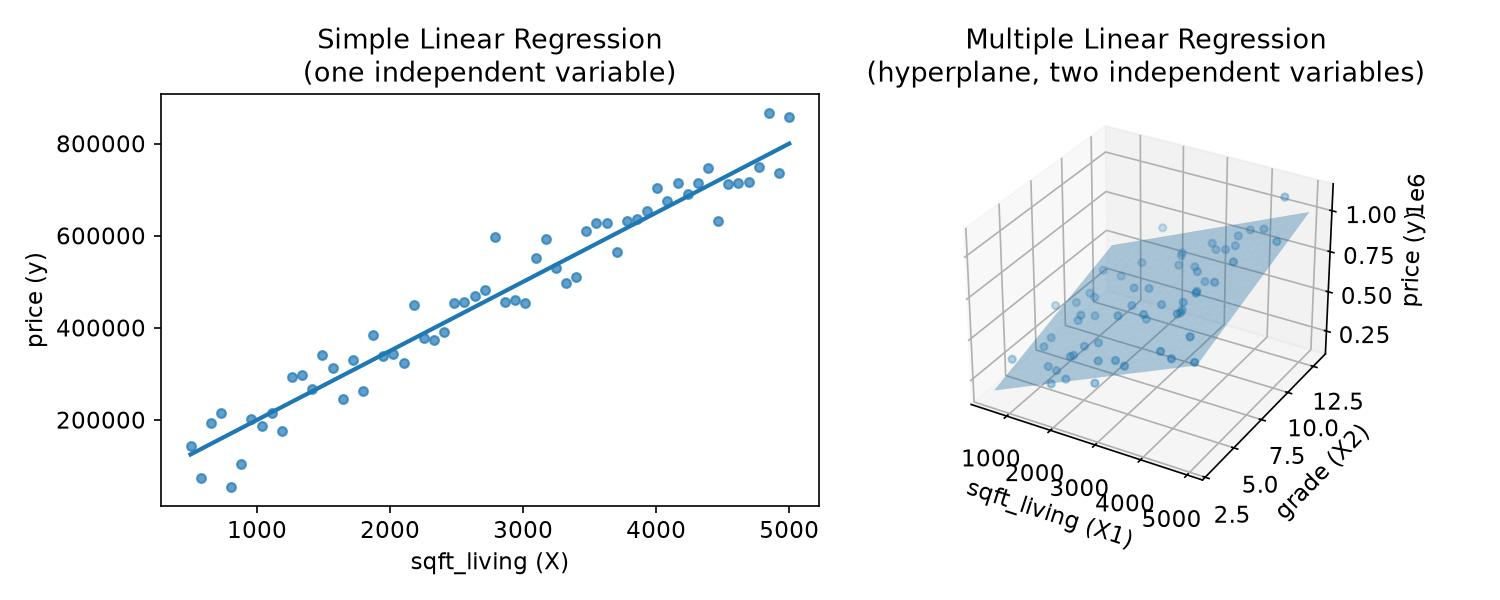
\includegraphics[width=0.9\textwidth]{images/regresi-linear-sederhana-vs-multipel.jpg}}
    \caption{Simple Linear Regression (satu variabel independen, garis lurus 2D) versus Multiple Linear Regression (dua variabel independen, bidang hyperplane 3D).}
    \label{fig:simple-vs-multiple}
\end{figure}

Secara matematis, model regresi linier berganda ditulis sebagai:
\begin{equation}
y = b_0 + b_1x_1 + b_2x_2 + \dots + b_nx_n
\end{equation}
di mana $b_0$ adalah \textit{intercept} (nilai dasar ketika semua fitur nol), $b_n$ adalah koefisien regresi yang menunjukkan pengaruh fitur $x_n$ terhadap prediksi, dan $y$ adalah target. Model mencari koefisien terbaik menggunakan teknik \textit{Least Squares} (kuadrat terkecil), yaitu metode yang meminimalkan jumlah kuadrat \textit{error} \cite{sklearn-linear,aws-linear}.

\begin{figure}[H]
    \centering
    \fbox{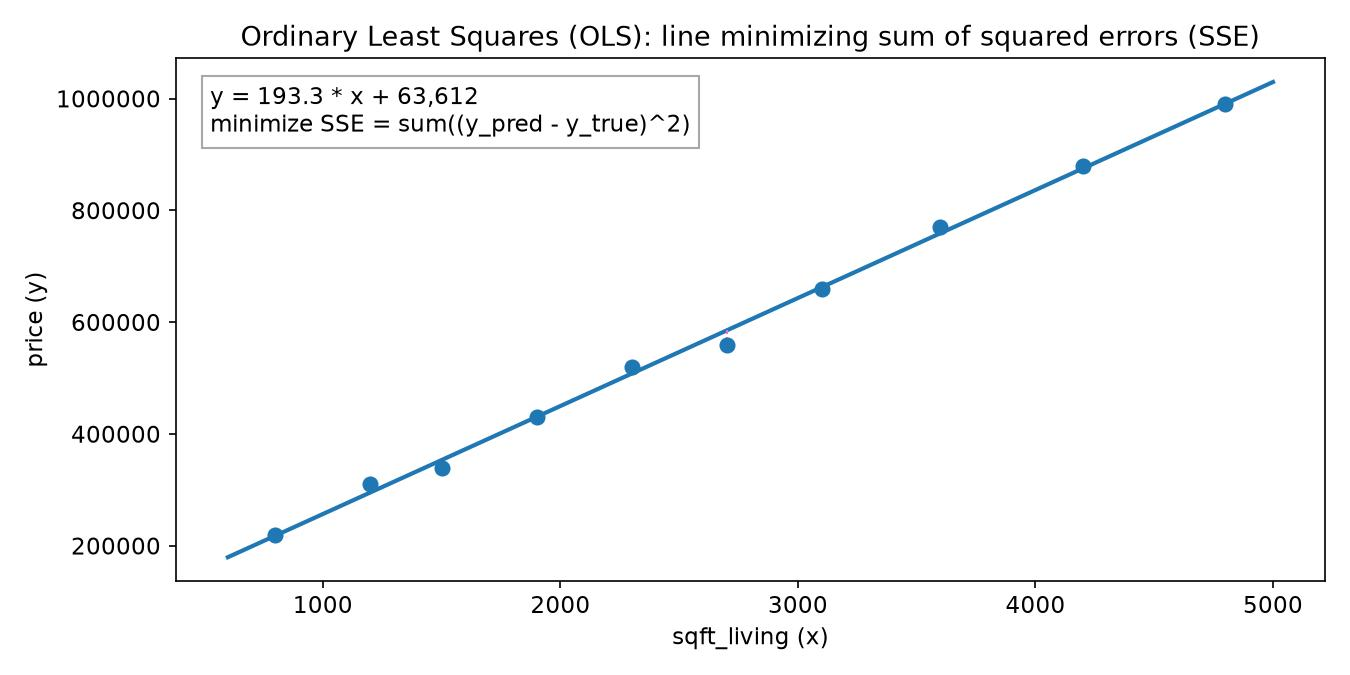
\includegraphics[width=0.9\textwidth]{images/ordinary-least-squares.jpg}}
    \caption{Ordinary Least Squares (OLS): garis optimal yang memberikan nilai sum of squared errors (SSE) terendah; garis putus-putus menunjukkan residual tiap titik data.}
    \label{fig:ols}
\end{figure}

Kelebihan Linear Regression adalah sangat cepat dan efisien untuk dataset besar, mudah dipahami dan dijelaskan (\textit{interpretable}), serta cocok untuk hubungan yang mendekati linear. Kekurangannya adalah kurang cocok untuk pola non-linear dan sensitif terhadap \textit{outlier}. Karena model memberi koefisien pada semua fitur termasuk yang daya prediksinya rendah, ia cenderung bersifat \textit{high-variance, low bias}, sehingga solusinya adalah regularisasi (Lasso, Ridge, Elastic Net) yang memberi penalti pada besarnya koefisien \cite{sklearn-linear,aws-linear}.

\begin{figure}[H]
    \centering
    \fbox{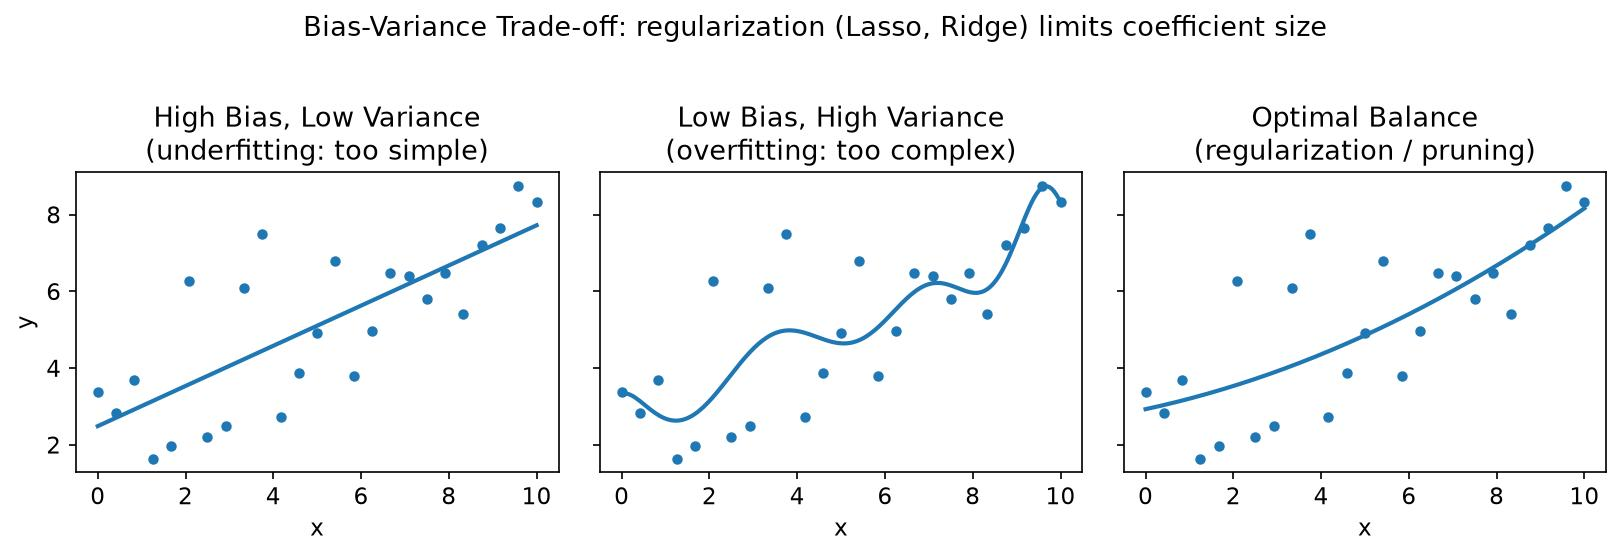
\includegraphics[width=0.9\textwidth]{images/bias-variance-tradeoff.jpg}}
    \caption{Bias-variance trade-off: model terlalu sederhana mengalami underfitting (high bias), model terlalu kompleks mengalami overfitting (low bias, high variance); regularisasi membantu mencapai keseimbangan optimal.}
    \label{fig:bias-variance}
\end{figure}

\subsection{Decision Tree Regression}
Decision Tree Regression bekerja dengan membangun struktur pohon keputusan sebagai representasi model. Algoritma ini membagi data menjadi beberapa subset berdasarkan titik \textit{split} yang dianggap paling optimal dalam mengurangi \textit{error}. Setiap pembagian \textit{node} dilakukan secara rekursif hingga mencapai \textit{leaf node} yang berisi nilai prediksi. Pemilihan \textit{split} biasanya dilakukan berdasarkan pengukuran \textit{error} seperti \textit{Mean Squared Error} (MSE), sehingga pemisahan data menghasilkan kelompok dengan variasi nilai target yang lebih homogen \cite{sklearn-tree,han2022,itbox-algoritma}.

Decision Tree Regression sangat efektif untuk memodelkan hubungan non-linear karena struktur pohon memungkinkan model membuat batas keputusan yang kompleks. Selain itu, decision tree tidak memerlukan normalisasi atau \textit{scaling} data dan dapat menangani fitur numerik maupun kategorikal. Kelemahan utamanya adalah kecenderungan \textit{overfitting}, yaitu ketika model terlalu menyesuaikan diri dengan data \textit{training} sehingga performanya menurun pada data baru. Solusinya adalah pembatasan kedalaman pohon (\texttt{max\_depth}) atau \textit{pruning} (pemangkasan pohon) \cite{sklearn-tree}.

\subsection{Random Forest Regression}
Random Forest Regression merupakan pengembangan dari Decision Tree yang menggunakan pendekatan \textit{ensemble learning}, yaitu membangun banyak pohon keputusan dan menggabungkan prediksinya. Setiap pohon dibangun menggunakan sampel data yang dipilih secara acak melalui \textit{bootstrap sampling}, serta subset fitur yang juga dipilih secara acak pada setiap pemisahan \textit{node}. Proses ini menciptakan berbagai variasi pohon yang kemudian memberikan hasil prediksi lebih stabil dan tidak mudah \textit{overfitting} dibanding \textit{tree} tunggal \cite{sklearn-ensemble,itbox-algoritma}.

Prediksi akhir pada Random Forest diperoleh dari rata-rata hasil prediksi semua pohon (untuk kasus regresi; pada klasifikasi memakai voting mayoritas), sehingga model mampu menangkap pola kompleks tanpa mengorbankan akurasi. Selain itu, Random Forest menyediakan informasi mengenai \textit{feature importance}, yang menunjukkan fitur mana yang paling berpengaruh dalam proses prediksi. Hal ini membuat Random Forest menjadi salah satu algoritma regresi yang umum digunakan, terutama pada dataset yang besar dan memiliki banyak fitur, meski memerlukan sumber daya komputasi yang lebih besar \cite{sklearn-ensemble}.

\section{Metrik Evaluasi Regression}
Dalam \textit{machine learning} khususnya pada model regresi, diperlukan metrik evaluasi untuk menilai seberapa baik model mampu memprediksi nilai numerik dengan tepat. Evaluasi ini dilakukan dengan membandingkan hasil prediksi model terhadap nilai aktual menggunakan metrik khusus regresi \cite{sklearn-metrics}.

\subsection{RMSE (Root Mean Squared Error)}
RMSE mengukur rata-rata jarak antara nilai prediksi dan nilai sebenarnya dengan memberikan penalti lebih besar terhadap kesalahan yang besar. RMSE merupakan akar dari \textit{Mean Squared Error}, sehingga unitnya sama dengan unit target dan lebih mudah diinterpretasikan dalam masalah nyata. Nilai RMSE yang lebih kecil menandakan bahwa model menghasilkan prediksi yang lebih akurat \cite{sklearn-metrics}.
\begin{equation}
RMSE = \sqrt{\frac{1}{n}\sum(y_{pred} - y_{true})^2}
\end{equation}
Karena RMSE memberikan penalti lebih besar pada kesalahan ekstrem, metrik ini sensitif terhadap \textit{outlier}. Sensitivitas tersebut justru menjadikan RMSE cocok digunakan pada data kontinu seperti harga rumah, di mana perbedaan nilai yang besar memberikan dampak signifikan terhadap evaluasi performa model.

\subsection{Coefficient of Determination (R\textsuperscript{2})}
\textit{Coefficient of Determination} atau R\textsuperscript{2} menunjukkan seberapa besar proporsi variansi target yang dapat dijelaskan oleh model. Nilai R\textsuperscript{2} berada pada rentang 0 hingga 1, di mana nilai mendekati 1 menandakan bahwa model memiliki kemampuan prediksi yang baik dan dapat menangkap pola hubungan dengan baik \cite{sklearn-metrics}.
\begin{equation}
R^2 = 1 - \frac{SS_{res}}{SS_{tot}}
\end{equation}

\begin{figure}[H]
    \centering
    \fbox{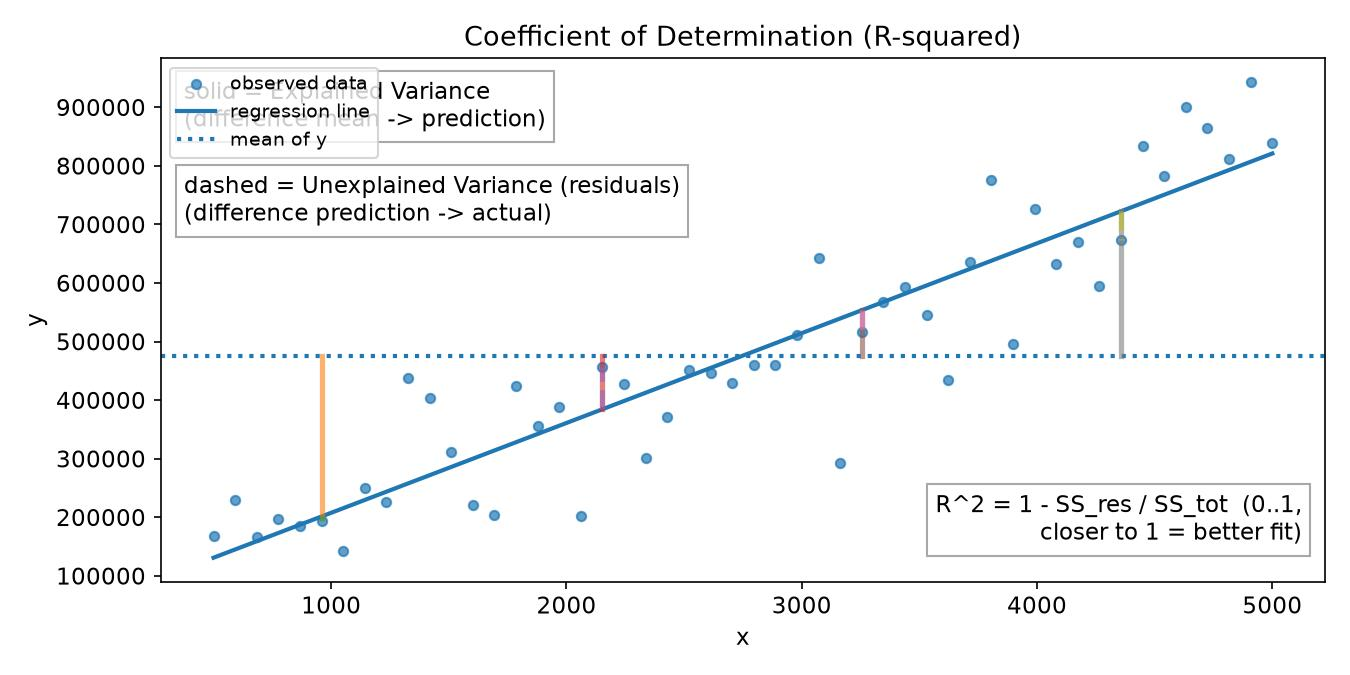
\includegraphics[width=0.9\textwidth]{images/koefisien-determinasi-r2.jpg}}
    \caption{Koefisien determinasi (R\textsuperscript{2}): proporsi explained variance (selisih rata-rata ke prediksi) terhadap total variance; sisanya adalah unexplained variance (residual).}
    \label{fig:r2}
\end{figure}

Nilai R\textsuperscript{2} yang semakin mendekati 1 menunjukkan bahwa model mampu menjelaskan proporsi variansi target dengan lebih baik. Sebaliknya, jika nilai R\textsuperscript{2} rendah, berarti model kurang mampu menangkap hubungan antara fitur dan target. Perlu dicatat bahwa R\textsuperscript{2} pada data \textit{training} dan \textit{testing} sebaiknya dibandingkan: selisih yang besar mengindikasikan \textit{overfitting} \cite{sklearn-metrics,han2022}.

\subsection{Koefisien Korelasi Pearson (R)}
Koefisien korelasi Pearson ($r$) mengukur kekuatan dan arah hubungan linier antara dua variabel, dalam hal ini antara nilai prediksi dan nilai sebenarnya. Nilainya berada pada rentang $-1$ hingga $1$: semakin dekat ke 1, semakin kuat hubungan linier positif antara prediksi dan aktual, yang berarti model semakin baik \cite{sklearn-metrics}.

\subsection{Mengapa Tidak Memakai Accuracy, Precision, Recall?}
Metrik seperti \textit{accuracy}, \textit{precision}, dan \textit{recall} dirancang untuk target diskrit berbasis \textit{confusion matrix} (TP, TN, FP, FN). Pada regresi, prediksi berupa bilangan kontinu sehingga peluang prediksi sama persis dengan nilai aktual praktis nol dan konsep benar/salah tidak terdefinisi. Oleh karena itu, performa model regresi harus diukur dari besarnya \textit{error} (RMSE) dan proporsi variansi yang dijelaskan model (R\textsuperscript{2}), bukan dari proporsi prediksi yang tepat \cite{sklearn-metrics}.

\section{Validation Techniques}
Performa model dapat dipengaruhi oleh ukuran data latih dan uji. Teknik validasi umum yang dipakai pada praktikum ini adalah \textit{holdout}: data dibagi menjadi training set (70\%) dan testing set (30\%). Model dilatih pada training set dan dievaluasi pada testing set yang tidak pernah dilihat selama pelatihan. Parameter \texttt{random\_state=42} dipakai agar pembagian data tetap konsisten setiap kali kode dijalankan \cite{han2022,dicoding-workflow,digitalskola-preprocessing}.

\clearpage

\chapter[\tocboldsection{Hasil dan Pembahasan}]{Hasil dan Pembahasan}

\section{Percobaan Latihan Praktikum}
Pada bagian ini saya mendokumentasikan percobaan regresi sesuai langkah pada Modul Pertemuan 4. Dataset yang digunakan adalah \textit{KC House Data} dari Kaggle~\cite{kaggle-kc} (\url{https://www.kaggle.com/datasets/shivachandel/kc-house-data}) yang juga tersedia di GitHub \texttt{ganjar87/data\_science\_practice}. Dataset ini berisi data penjualan rumah di King County (termasuk Seattle, AS) dari Mei 2014 sampai Mei 2015. Setiap langkah disertai kode yang saya jalankan di Google Colaboratory beserta screenshot hasil eksekusinya. Notebook yang saya gunakan adalah \texttt{praktikum-4-regression.ipynb} pada repositori PPD, yang siap diimpor ke Google Colaboratory melalui \texttt{colab.research.google.com/github}.

\subsection{Alat dan Bahan}
Sesuai Modul 4.3, alat dan bahan yang saya gunakan adalah:
\begin{itemize}
    \item \textbf{Perangkat keras:} Laptop/komputer dengan akses internet.
    \item \textbf{Perangkat lunak:} Python~3~\cite{python-docs} dan Google Colaboratory sebagai lingkungan eksekusi notebook. Pustaka utama yang saya gunakan meliputi pandas~\cite{pandas-docs}, NumPy~\cite{numpy-docs}, Matplotlib, Seaborn, dan Scikit-Learn untuk pemodelan regresi \cite{sklearn-metrics,sklearn-preprocessing}.
\end{itemize}
Dataset KC House saya akses melalui mirror GitHub agar dapat dimuat langsung dengan \texttt{pd.read\_csv()} tanpa unduhan manual dari Kaggle, sedangkan dataset tugas Car Price saya akses melalui mirror \texttt{SampattKumar/Linear-Regression-Car-Dataset} di GitHub.

\subsection{Persiapan dan Impor Pustaka}
Saya menyiapkan lingkungan Python~\cite{python-docs} dan mengimpor pustaka yang dibutuhkan untuk manipulasi data dengan pandas~\cite{pandas-docs}, komputasi numerik dengan NumPy~\cite{numpy-docs}, visualisasi, serta pemodelan regresi (Linear Regression, Decision Tree, Random Forest) beserta metrik evaluasinya.

\begin{lstlisting}[style=pythonstyle,caption={Impor pustaka praktikum regresi.}]
import pandas as pd
import numpy as np
import matplotlib.pyplot as plt
import seaborn as sns

from sklearn.model_selection import train_test_split
from sklearn.linear_model import LinearRegression
from sklearn.tree import DecisionTreeRegressor
from sklearn.ensemble import RandomForestRegressor
from sklearn.metrics import mean_squared_error, r2_score
\end{lstlisting}

\begin{figure}[H]
\centering
\customfbox{
\includegraphics[width=0.9\textwidth]{images/ss-01-import-library.jpg}}
\caption{Impor pustaka yang digunakan dalam praktikum regresi.}
\label{fig:ss01-import}
\end{figure}

\subsection{Memuat Dataset KC House}
Saya memuat dataset KC House yang berisi 21.613 baris dengan 21 kolom, meliputi atribut properti (luas, kamar, grade, lokasi) dan target \texttt{price} (harga rumah).

\begin{lstlisting}[style=pythonstyle,caption={Memuat dataset KC House.}]
df = pd.read_csv('https://raw.githubusercontent.com/ganjar87/data_science_practice/main/kc_house_data.csv')
print(df.shape)  # (21613, 21)
df.head()
\end{lstlisting}

\begin{figure}[H]
\centering
\customfbox{
\includegraphics[width=0.9\textwidth]{images/ss-02-dataset-head.jpg}}
\caption{Lima baris pertama dataset KC House: kolom \texttt{id}, \texttt{date}, \texttt{price}, \texttt{bedrooms}, \texttt{bathrooms}, \texttt{sqft\_living}, hingga \texttt{grade} dan \texttt{sqft\_above}.}
\label{fig:ss02-head}
\end{figure}

\begin{lstlisting}[style=pythonstyle,caption={Lima baris terakhir dataset.}]
df.tail()
\end{lstlisting}

\begin{figure}[H]
\centering
\customfbox{
\includegraphics[width=0.9\textwidth]{images/ss-03-dataset-tail.jpg}}
\caption{Lima baris terakhir dataset dengan struktur kolom yang sama, memberikan gambaran variasi data di akhir kumpulan dataset.}
\label{fig:ss03-tail}
\end{figure}

\subsection{Exploratory Data Analysis (EDA)}

\subsubsection{Deskripsi Statistik}
Saya melihat deskripsi statistik untuk memahami sebaran variabel numerik. Rata-rata harga rumah (\texttt{price}) sekitar 540.088 dengan rata-rata luas bangunan (\texttt{sqft\_living}) sekitar 2.079. Standar deviasi \texttt{price} yang besar menandakan sebaran harga yang lebar, termasuk rumah-rumah yang sangat mahal.

\begin{lstlisting}[style=pythonstyle,caption={Deskripsi statistik dataset.}]
display(df.describe())
\end{lstlisting}

\begin{figure}[H]
\centering
\customfbox{
\includegraphics[width=0.9\textwidth]{images/ss-04-describe.jpg}}
\caption{Hasil deskripsi statistik: baris metrik (count, mean, std, min, 25\%, 50\%, 75\%, max) untuk variabel numerik seperti \texttt{price}, \texttt{bedrooms}, \texttt{bathrooms}, dan \texttt{sqft\_living}.}
\label{fig:ss04-describe}
\end{figure}

\subsubsection{Histogram Variabel Numerik}
Saya memplot histogram untuk melihat distribusi tiap variabel numerik. Histogram \texttt{price} sangat condong ke kanan (\textit{right-skewed}) dengan banyak outlier di nilai tinggi, sementara \texttt{bedrooms} dan \texttt{bathrooms} menunjukkan distribusi diskrit yang terkonsentrasi pada nilai-nilai kecil.

\begin{lstlisting}[style=pythonstyle,caption={Kode untuk menampilkan histogram.}]
# check histogram for continuous columns
df.hist(figsize=(10,10))
plt.tight_layout()
plt.show()
\end{lstlisting}

\begin{figure}[H]
\centering
\customfbox{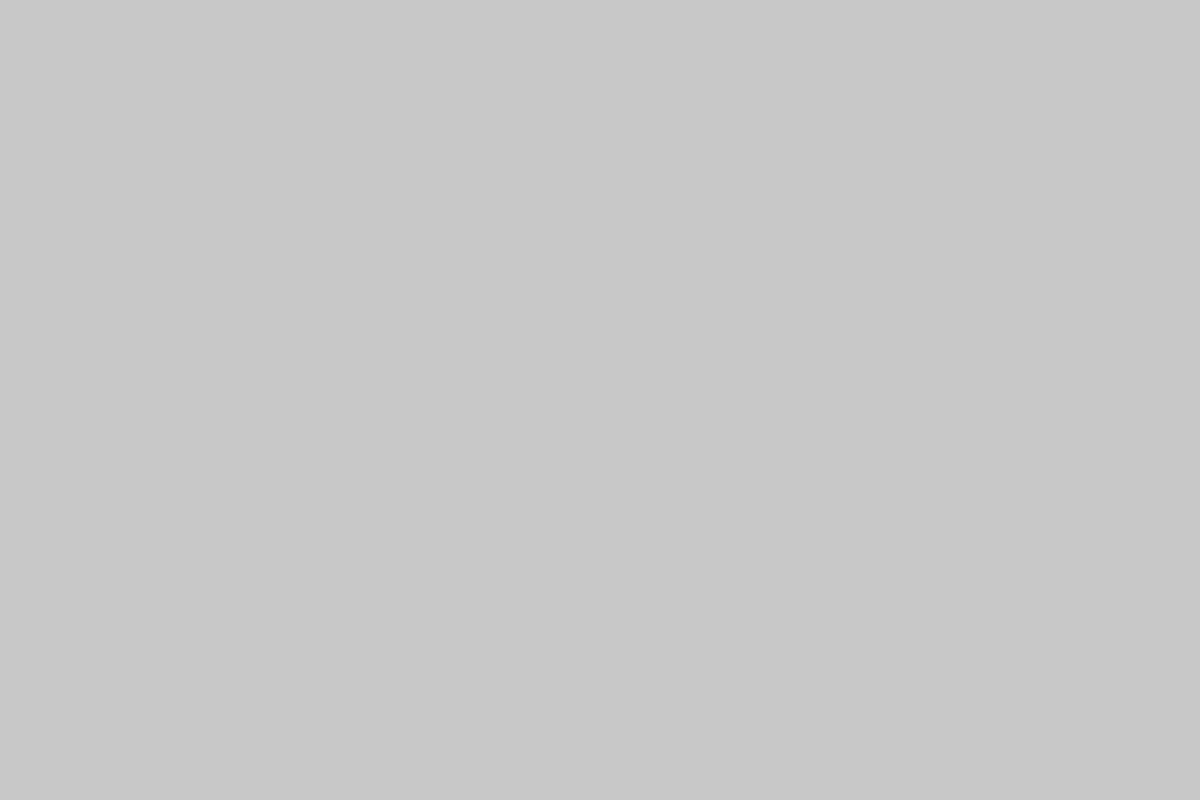
\includegraphics[width=0.7\textwidth]{images/ss-05-histogram-code.jpg}}
\caption{Kode untuk memplot histogram setiap kolom numerik dengan fungsi bawaan pandas/matplotlib.}
\label{fig:ss05-histcode}
\end{figure}

\begin{figure}[H]
\centering
\customfbox{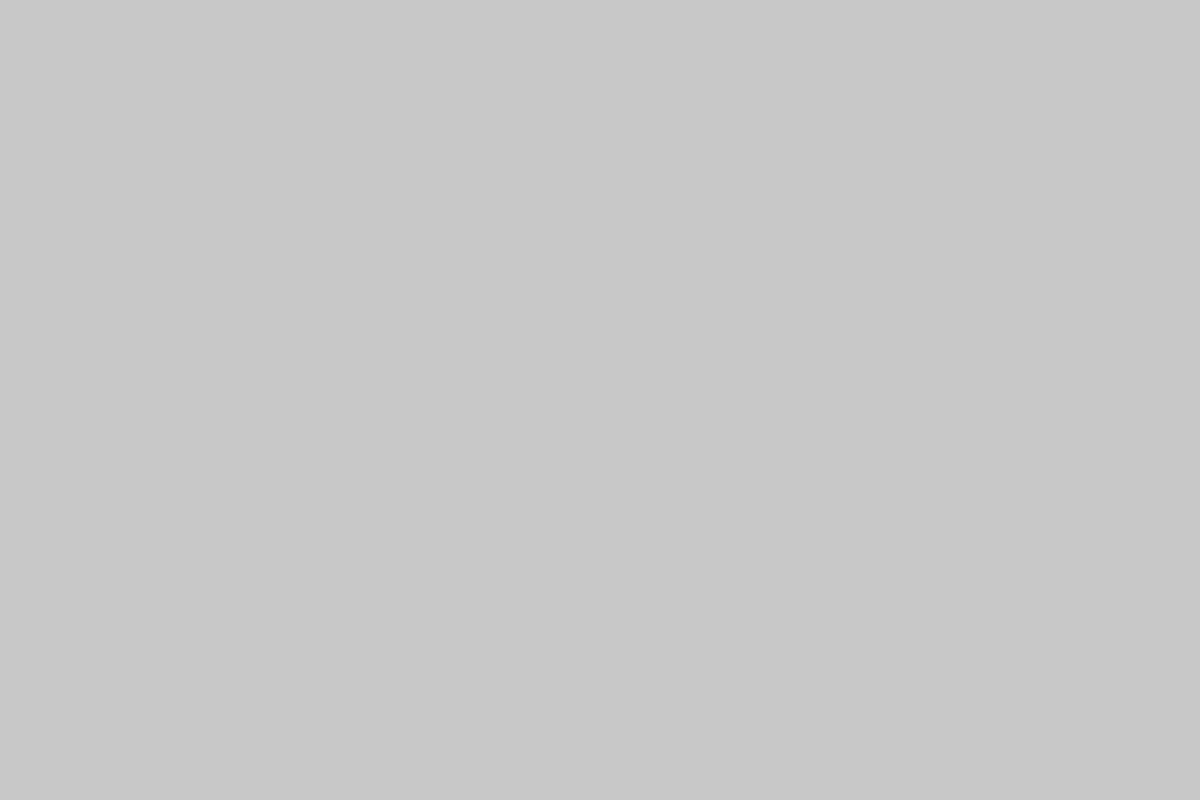
\includegraphics[width=0.9\textwidth]{images/ss-06-histogram-result.jpg}}
\caption{Grid histogram seluruh variabel numerik: \texttt{price} right-skewed, variabel diskrit menumpuk di nilai kecil.}
\label{fig:ss06-histresult}
\end{figure}

\subsubsection{Korelasi Atribut Numerik}
Saya mengecek matriks korelasi Pearson antar variabel numerik. Korelasi positif terkuat dengan \texttt{price} adalah \texttt{sqft\_living} (0,70), \texttt{grade} (0,67), dan \texttt{sqft\_above} (0,61): semakin luas dan semakin tinggi grade rumah, semakin tinggi harganya.

\begin{lstlisting}[style=pythonstyle,caption={Korelasi atribut numerik.}]
# check correlation coef
display(df.corr(numeric_only=True))
\end{lstlisting}

\begin{figure}[H]
\centering
\customfbox{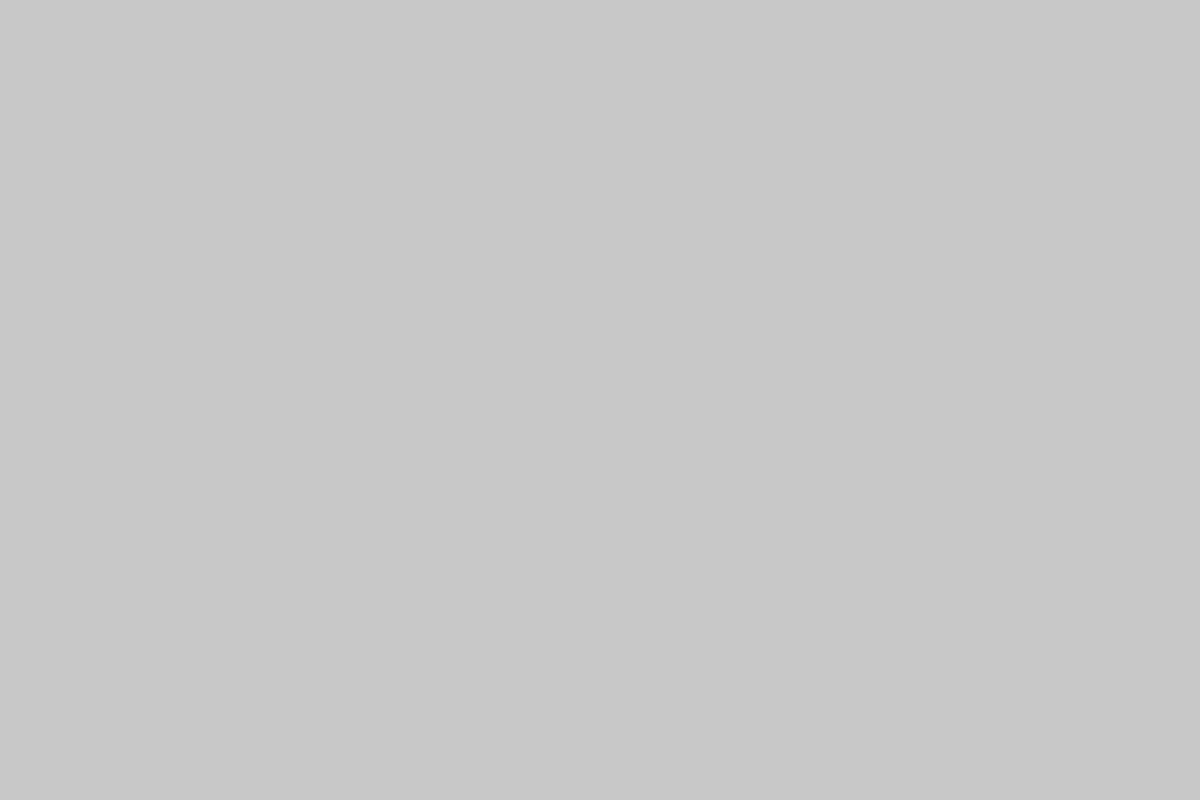
\includegraphics[width=0.9\textwidth]{images/ss-07-korelasi.jpg}}
\caption{Matriks korelasi Pearson antar seluruh variabel numerik.}
\label{fig:ss07-corr}
\end{figure}

\subsubsection{Pengecekan Missing Value}
Saya mengecek nilai kosong di seluruh kolom. Hasilnya seluruh kolom memiliki 0 nilai kosong, sehingga dataset sudah bersih dan bisa langsung dipakai untuk pemodelan tanpa imputasi.

\begin{lstlisting}[style=pythonstyle,caption={Pengecekan missing value.}]
print(df.isnull().sum())
\end{lstlisting}

\begin{figure}[H]
\centering
\customfbox{
\includegraphics[width=0.7\textwidth]{images/ss-08-missing-value.jpg}}
\caption{Hasil pengecekan missing value: seluruh kolom 0 nilai kosong.}
\label{fig:ss08-missing}
\end{figure}

\subsubsection{Pengecekan Atribut Kategorikal}
Saya mengecek kolom bertipe objek/kategorikal. Setelah kolom \texttt{id}, \texttt{date}, dan \texttt{price} dibuang, hasilnya adalah Index kosong: tidak ada lagi kolom bertipe objek atau boolean, sehingga semua fitur sudah numerik dan tidak memerlukan encoding.

\begin{lstlisting}[style=pythonstyle,caption={Pengecekan atribut kategorikal.}]
df_X = df.drop(['id', 'date', 'price'], axis=1)
df_y = df['price']
cats = df_X.select_dtypes(include=['object', 'bool']).columns
print(cats)
\end{lstlisting}

\begin{figure}[H]
\centering
\customfbox{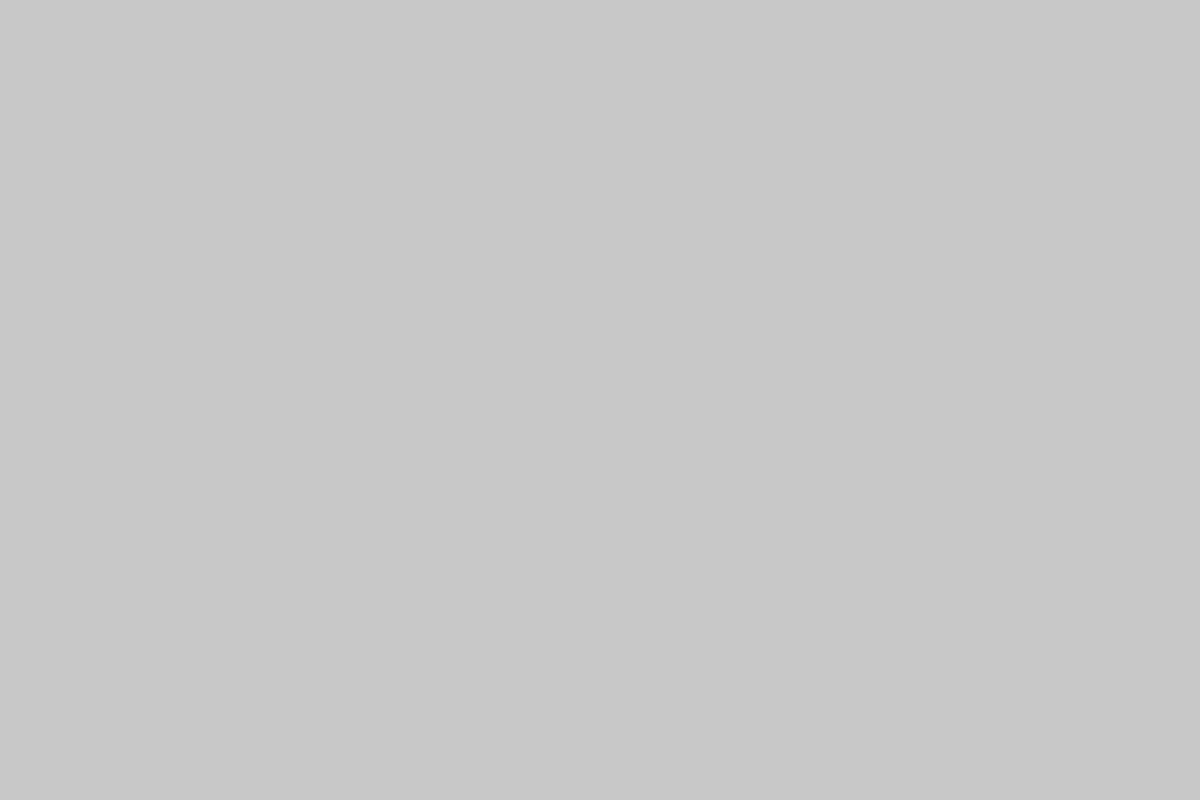
\includegraphics[width=0.7\textwidth]{images/ss-09-kategorikal.jpg}}
\caption{Hasil pengecekan atribut kategorikal: tidak ada kolom objek/boolean yang tersisa.}
\label{fig:ss09-cats}
\end{figure}

\subsection{Modelling}

\subsubsection{a. Linear Regression}
Proses pemodelan saya mulai dengan menentukan fitur dan target: \texttt{df\_X} dibuat dengan menghapus kolom \texttt{id}, \texttt{date}, dan \texttt{price} karena \texttt{price} menjadi target prediksi sedangkan \texttt{id} dan \texttt{date} tidak informatif. Kedua variabel diubah menjadi array numerik float, lalu data dibagi 70:30 dengan \texttt{random\_state=42}. Model \texttt{LinearRegression()} dilatih dengan \texttt{.fit()}, kemudian saya menghitung R\textsuperscript{2} training dan testing, melihat koefisien dan \textit{intercept}, serta memprediksi 10 data pertama untuk dibandingkan dengan nilai sebenarnya.

\begin{lstlisting}[style=pythonstyle,caption={Kode model Linear Regression.}]
from sklearn.linear_model import LinearRegression
from sklearn.model_selection import train_test_split

df_X = df.drop(['id','date','price'], axis=1)
df_y = df['price']

X = df_X.astype(float).values
y = df_y.astype(float).values

X_train, X_test, y_train, y_test = train_test_split(X, y, test_size=0.3, random_state=42)

reg = LinearRegression()
reg.fit(X_train, y_train)

print('coef of determination training', reg.score(X_train, y_train))
print('coef of determination testing', reg.score(X_test, y_test))

print('coefficient')
print(reg.coef_)
print('intercept')
print(reg.intercept_)

print('prediction')
y_pred = reg.predict(X_test)
print(y_pred[:10])
print('real value')
print(y_test[0:10])
\end{lstlisting}

\begin{figure}[H]
\centering
\customfbox{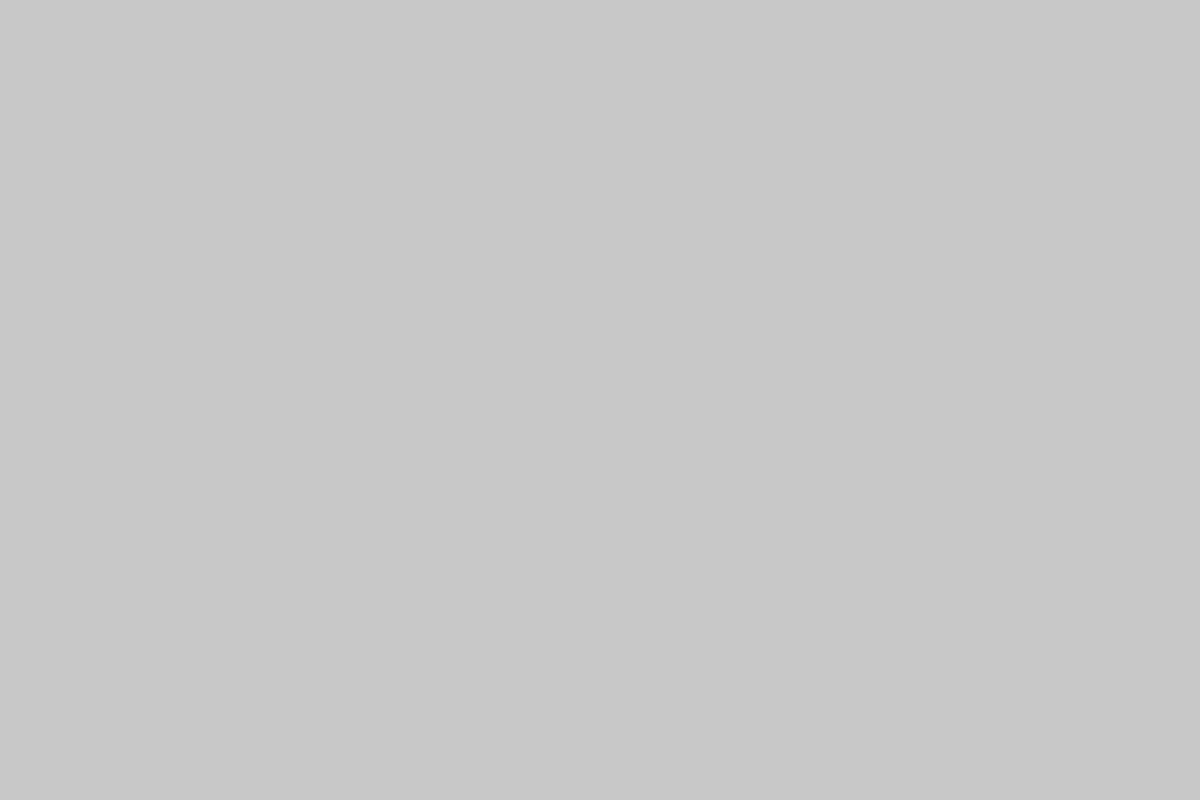
\includegraphics[width=0.9\textwidth]{images/ss-10-linear-code.jpg}}
\caption{Kode pemodelan Linear Regression: pemisahan fitur/target, split 70:30, training, skor R\textsuperscript{2}, koefisien, intercept, dan prediksi.}
\label{fig:ss10-lincode}
\end{figure}

Hasil training menunjukkan \textit{coef of determination training} 0,6995 dan \textit{testing} 0,6995 yang hampir identik, artinya model stabil dan tidak overfitting. Koefisien menunjukkan pengaruh masing-masing fitur terhadap harga, sedangkan \textit{intercept} sebesar 6.641.646,71 merupakan nilai dasar ketika semua fitur nol. Sepuluh prediksi pertama terlihat mendekati nilai sebenarnya meski ada selisih (error) pada beberapa sampel.

\begin{figure}[H]
\centering
\customfbox{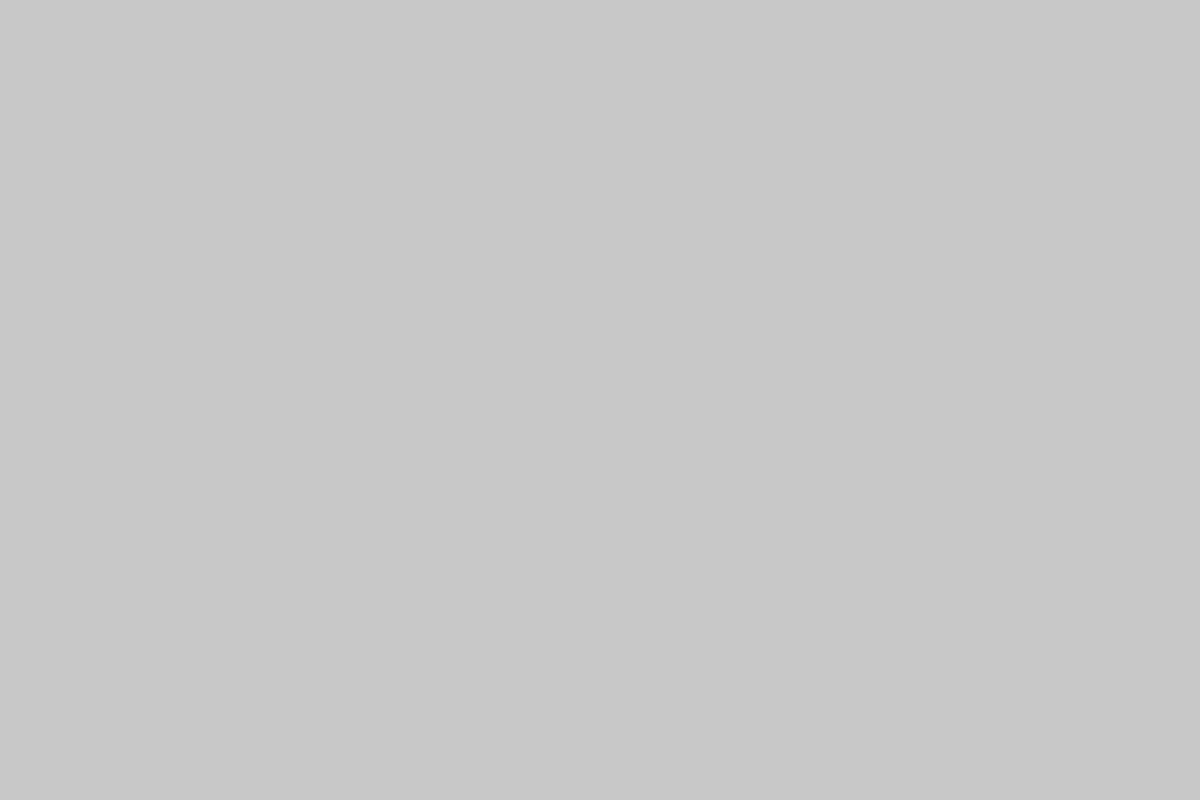
\includegraphics[width=0.9\textwidth]{images/ss-11-linear-train-output.jpg}}
\caption{Output pelatihan Linear Regression: skor R\textsuperscript{2} training/testing, koefisien, intercept, 10 prediksi pertama, dan 10 nilai sebenarnya.}
\label{fig:ss11-linout}
\end{figure}

Selanjutnya saya mengevaluasi model dengan RMSE dan R\textsuperscript{2}. MSE dihitung dengan \texttt{mean\_squared\_error}, diakarkan menjadi RMSE agar satuannya sama dengan dolar, dan R\textsuperscript{2} dihitung dengan \texttt{r2\_score}.

\begin{lstlisting}[style=pythonstyle,caption={Kode evaluasi Linear Regression.}]
from sklearn.metrics import mean_squared_error
from sklearn.metrics import r2_score
import numpy as np

mse = mean_squared_error(y_test, y_pred)
rmse = np.sqrt(mse)
r2 = r2_score(y_test, y_pred)

print('rmse:', rmse)
print('r2:', r2)
\end{lstlisting}

\begin{figure}[H]
\centering
\customfbox{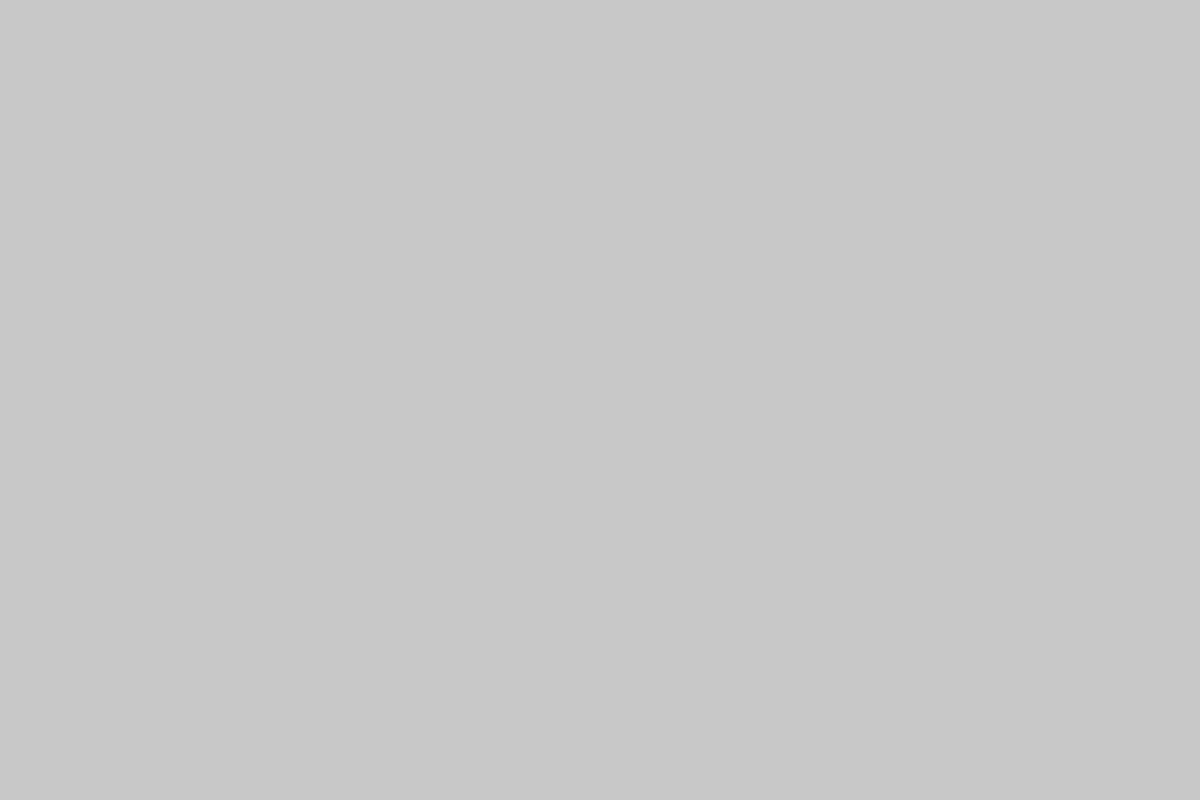
\includegraphics[width=0.7\textwidth]{images/ss-12-linear-eval-code.jpg}}
\caption{Kode evaluasi Linear Regression menggunakan RMSE dan R\textsuperscript{2}.}
\label{fig:ss12-linevalcode}
\end{figure}

Hasilnya RMSE sebesar 208.296,73 yang berarti rata-rata kesalahan prediksi model berada di kisaran angka tersebut terhadap harga sebenarnya, dan R\textsuperscript{2} sebesar 0,699 yang berarti model menjelaskan sekitar 69,9\% variansi harga rumah. Masih ada sekitar 30\% variansi yang belum dijelaskan model.

\begin{figure}[H]
\centering
\customfbox{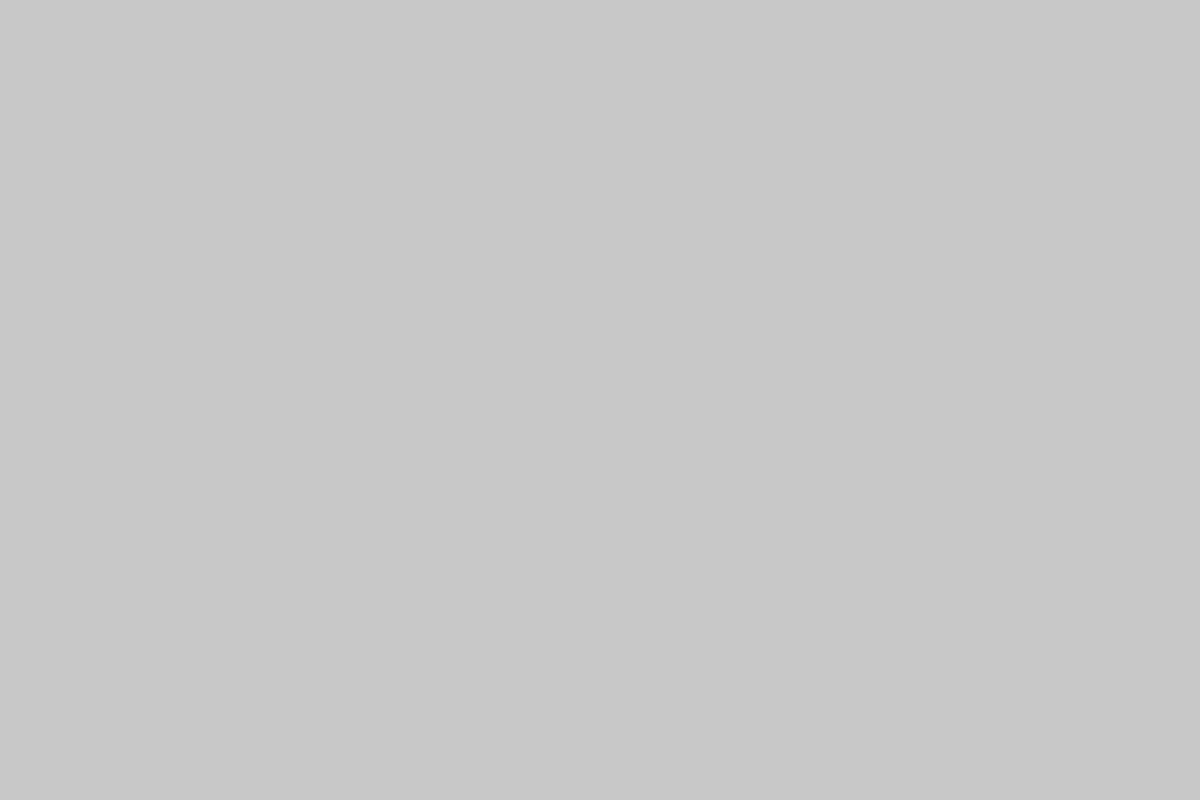
\includegraphics[width=0.7\textwidth]{images/ss-13-linear-eval-result.jpg}}
\caption{Hasil evaluasi Linear Regression: RMSE 208296,73 dan R\textsuperscript{2} 0,699.}
\label{fig:ss13-linevalres}
\end{figure}

Terakhir saya memvisualisasikan 50 sampel pertama dalam grafik batang untuk membandingkan nilai prediksi dan nilai sebenarnya. Pola batang prediksi secara umum mengikuti fluktuasi batang nilai sebenarnya, namun ada deviasi ketinggian pada beberapa titik yang merepresentasikan error prediksi.

\begin{lstlisting}[style=pythonstyle,caption={Kode visualisasi Linear Regression.}]
import seaborn as sns
import matplotlib.pyplot as plt

data1 = pd.Series(y_test[:50].ravel())
data2 = pd.Series(y_pred[:50].ravel())

df_new = pd.concat([data1, data2], keys=['real values', 'predicted values'], axis=1)
# df_new.plot.bar() # bisa pakai cara 1
df_new.plot(kind='bar', figsize=(15,3)) # bisa pakai cara 2

plt.title("Linear regression")
plt.xlabel('Sample i')
plt.ylabel('House Price')
plt.show()
\end{lstlisting}

\begin{figure}[H]
\centering
\customfbox{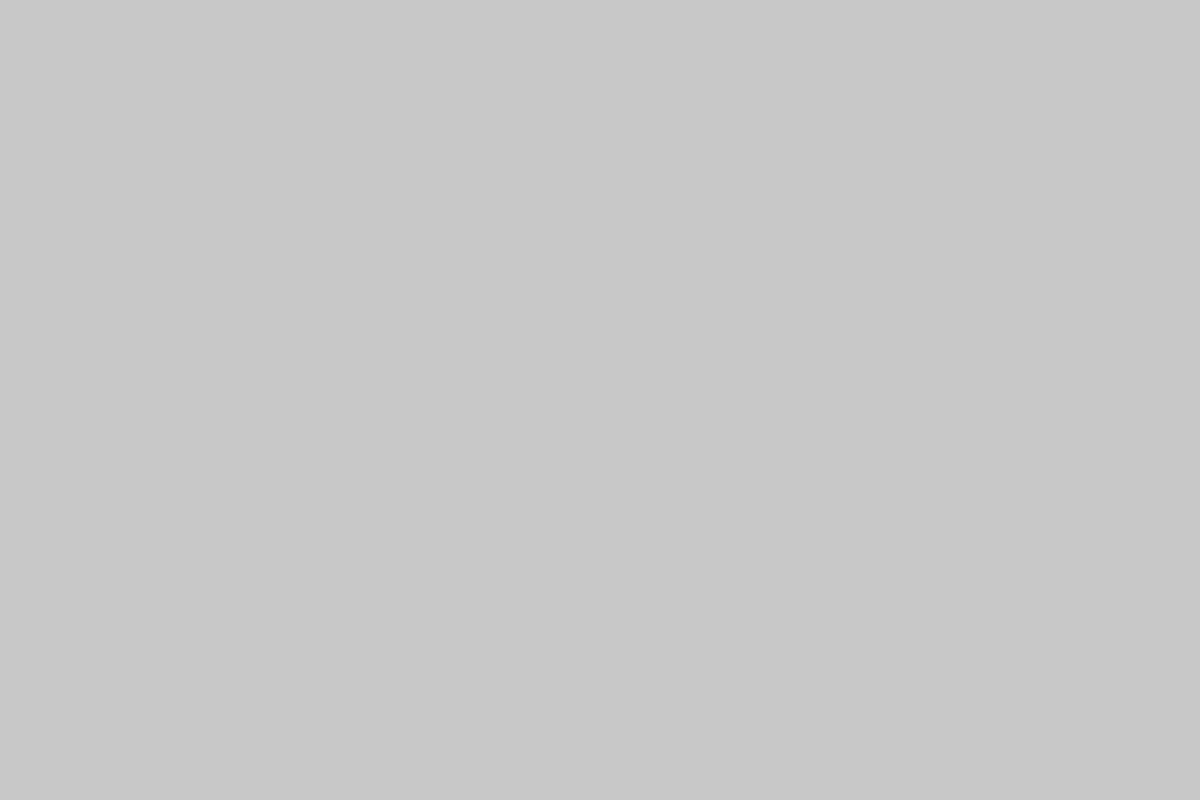
\includegraphics[width=0.9\textwidth]{images/ss-14-linear-viz-code.jpg}}
\caption{Kode visualisasi perbandingan 50 nilai aktual dan prediksi Linear Regression.}
\label{fig:ss14-linvizcode}
\end{figure}

\begin{figure}[H]
\centering
\customfbox{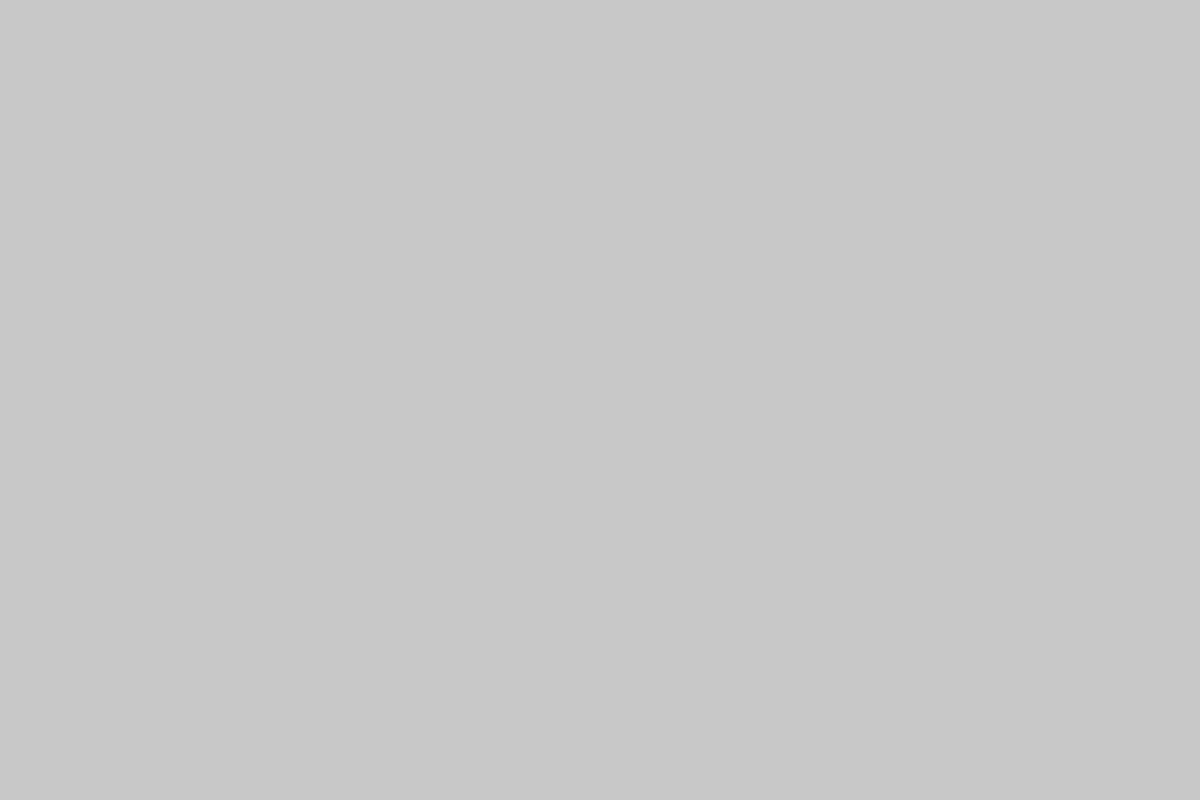
\includegraphics[width=0.9\textwidth]{images/ss-15-linear-viz-result.jpg}}
\caption{Grafik batang perbandingan \texttt{real values} dan \texttt{predicted values} untuk Linear Regression.}
\label{fig:ss15-linvizres}
\end{figure}

\subsubsection{b. Decision Tree Regression}
Untuk Decision Tree, langkah persiapan datanya identik, hanya modelnya yang diganti menjadi \texttt{DecisionTreeRegressor(max\_depth=10)}. Parameter \texttt{max\_depth=10} membatasi kedalaman maksimum pohon agar model tidak terlalu kompleks dan mengurangi risiko \textit{overfitting}.

\begin{lstlisting}[style=pythonstyle,caption={Kode model Decision Tree Regression.}]
from sklearn.tree import DecisionTreeRegressor
from sklearn.model_selection import train_test_split

df_X = df.drop(['id','date','price'], axis=1)
df_y = df['price']

X = df_X.astype(float).values
y = df_y.astype(float).values

X_train, X_test, y_train, y_test = train_test_split(X, y, test_size=0.3, random_state=42)

dt = DecisionTreeRegressor(max_depth=10)
dt.fit(X_train, y_train)

print('coef of determination training', dt.score(X_train, y_train))
print('coef of determination testing', dt.score(X_test, y_test))

print('prediction')
y_pred = dt.predict(X_test)
print(y_pred[:10])
print('real value')
print(y_test[0:10])
\end{lstlisting}

\begin{figure}[H]
\centering
\customfbox{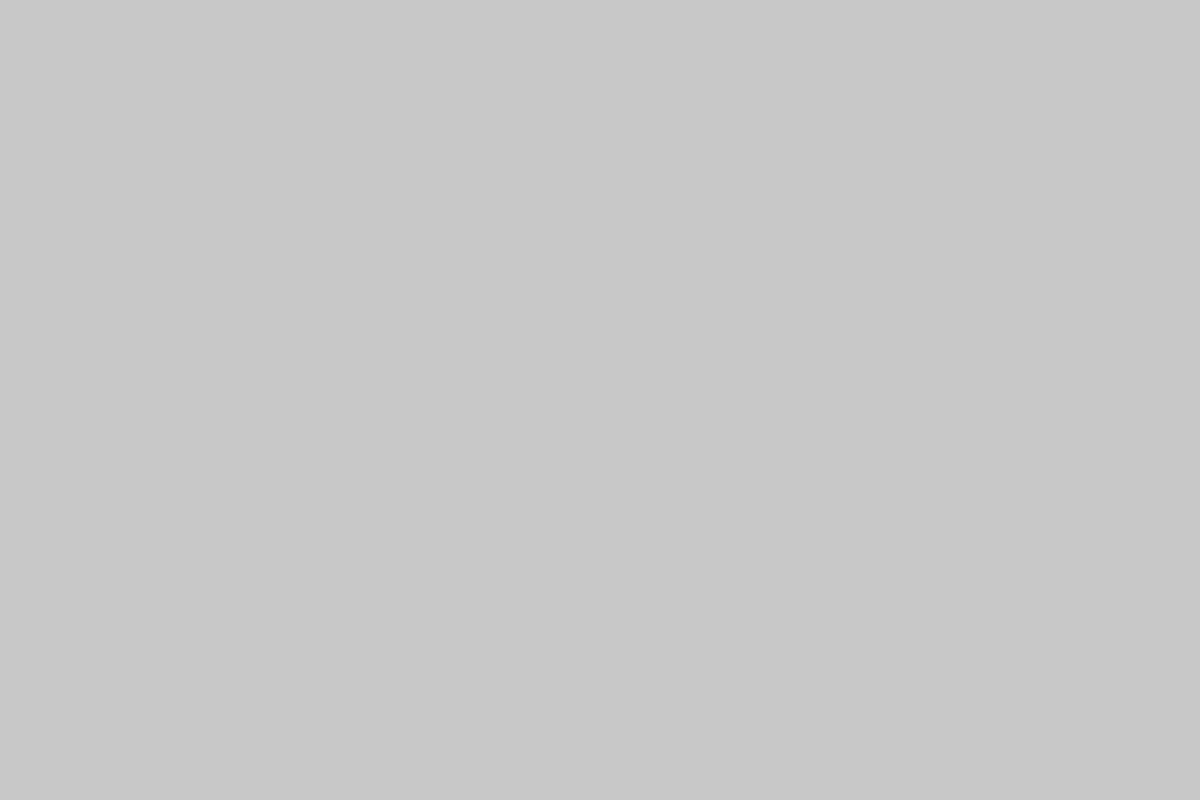
\includegraphics[width=0.9\textwidth]{images/ss-16-dt-code.jpg}}
\caption{Kode pemodelan Decision Tree Regression dengan \texttt{max\_depth=10}.}
\label{fig:ss16-dtcode}
\end{figure}

Hasilnya R\textsuperscript{2} training 0,9185 berbanding testing 0,7586: selisihnya cukup besar, yang menandakan pohon mulai overfitting meski kedalamannya sudah dibatasi.

\begin{figure}[H]
\centering
\customfbox{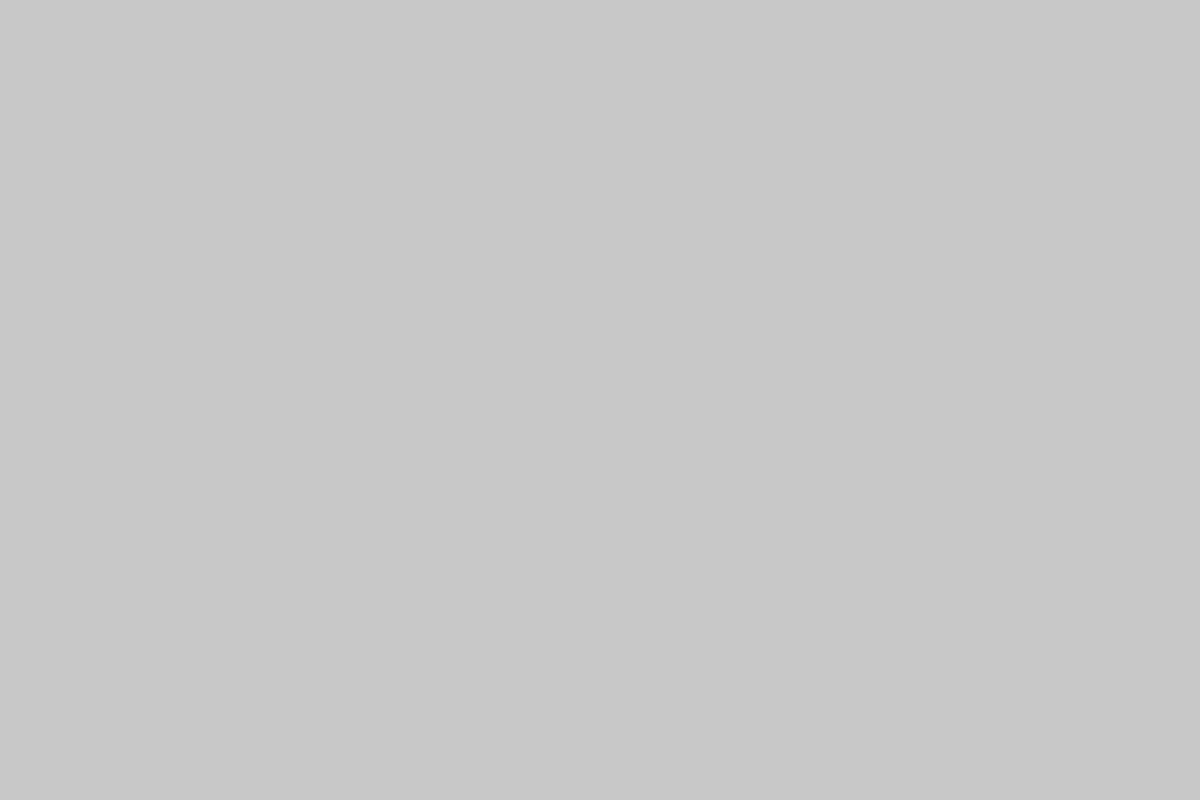
\includegraphics[width=0.9\textwidth]{images/ss-17-dt-output.jpg}}
\caption{Output pelatihan dan prediksi Decision Tree Regression.}
\label{fig:ss17-dtout}
\end{figure}

Evaluasi memakai kode yang identik dengan sebelumnya:

\begin{lstlisting}[style=pythonstyle,caption={Kode evaluasi Decision Tree.}]
from sklearn.metrics import mean_squared_error
from sklearn.metrics import r2_score
import numpy as np

mse = mean_squared_error(y_test, y_pred)
rmse = np.sqrt(mse)
r2 = r2_score(y_test, y_pred)

print('rmse:', rmse)
print('r2:', r2)
\end{lstlisting}

\begin{figure}[H]
\centering
\customfbox{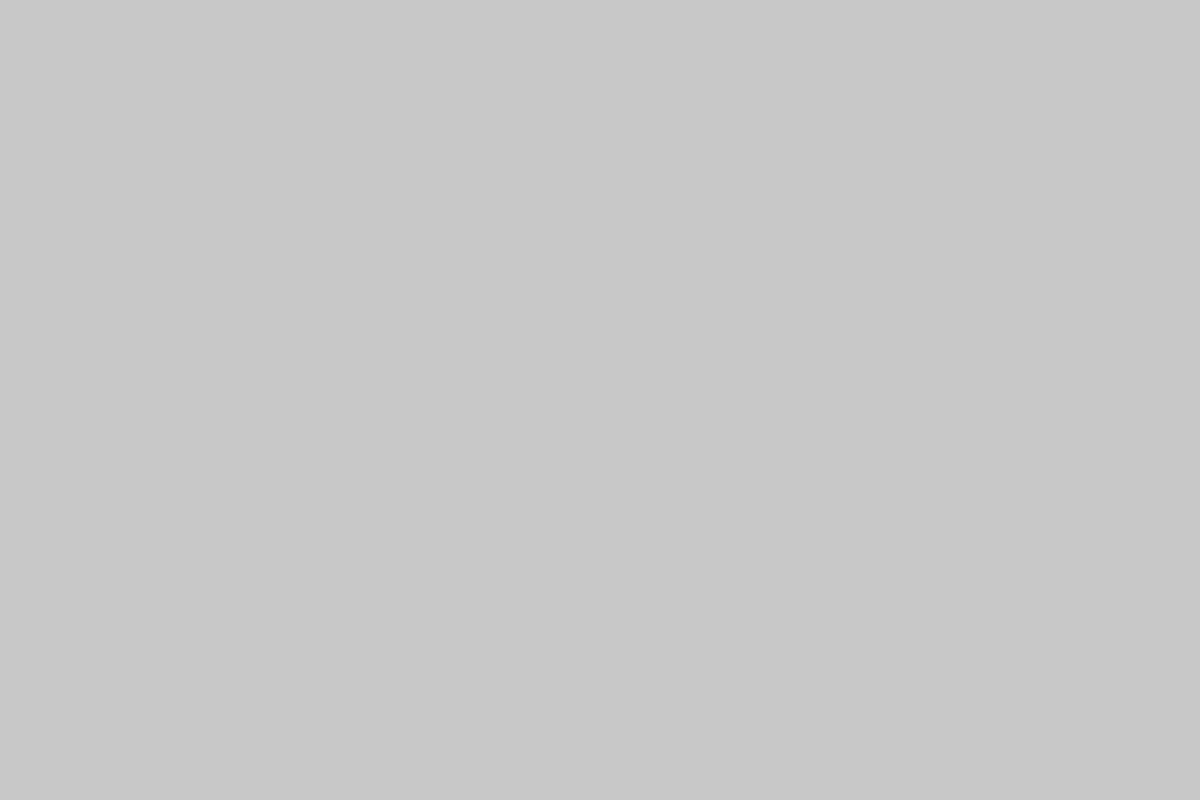
\includegraphics[width=0.7\textwidth]{images/ss-18-dt-eval-code.jpg}}
\caption{Kode evaluasi Decision Tree menggunakan RMSE dan R\textsuperscript{2}.}
\label{fig:ss18-dtevalcode}
\end{figure}

Hasilnya RMSE 184.751,00 dan R\textsuperscript{2} 0,7636: lebih baik dari Linear Regression karena struktur pohon mampu menangkap pola non-linear pada data.

\begin{figure}[H]
\centering
\customfbox{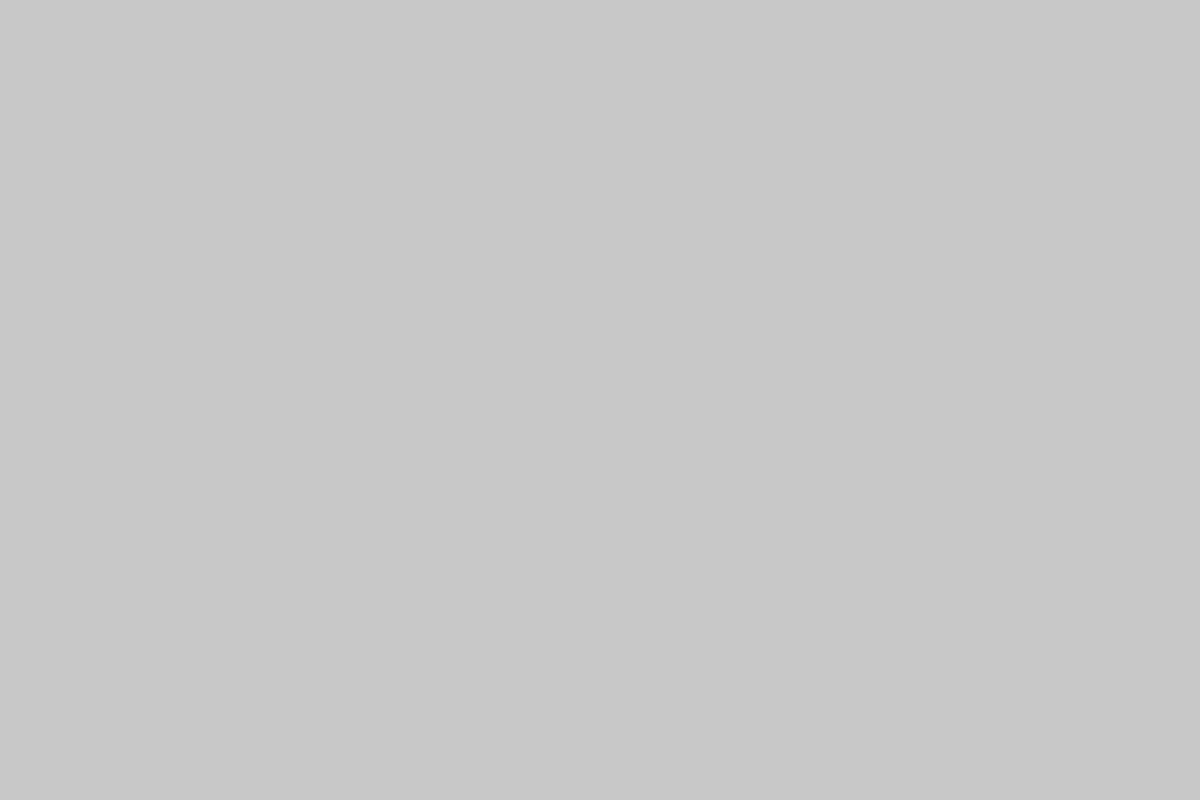
\includegraphics[width=0.7\textwidth]{images/ss-19-dt-eval-result.jpg}}
\caption{Hasil evaluasi Decision Tree: RMSE dan R\textsuperscript{2} lebih baik dibanding Linear Regression.}
\label{fig:ss19-dtevalres}
\end{figure}

Visualisasi 50 sampel menunjukkan batang prediksi lebih rapat mengikuti nilai sebenarnya dibanding Linear Regression, menandakan error yang lebih kecil pada beberapa titik.

\begin{lstlisting}[style=pythonstyle,caption={Kode visualisasi Decision Tree.}]
import seaborn as sns
import matplotlib.pyplot as plt

data1 = pd.Series(y_test[:50].ravel())
data2 = pd.Series(y_pred[:50].ravel())

df_new = pd.concat([data1, data2], keys=['real values', 'predicted values'], axis=1)
df_new.plot(kind='bar', figsize=(15,3))

plt.title("DT regression")
plt.xlabel('Sample i')
plt.ylabel('House Price')
plt.show()
\end{lstlisting}

\begin{figure}[H]
\centering
\customfbox{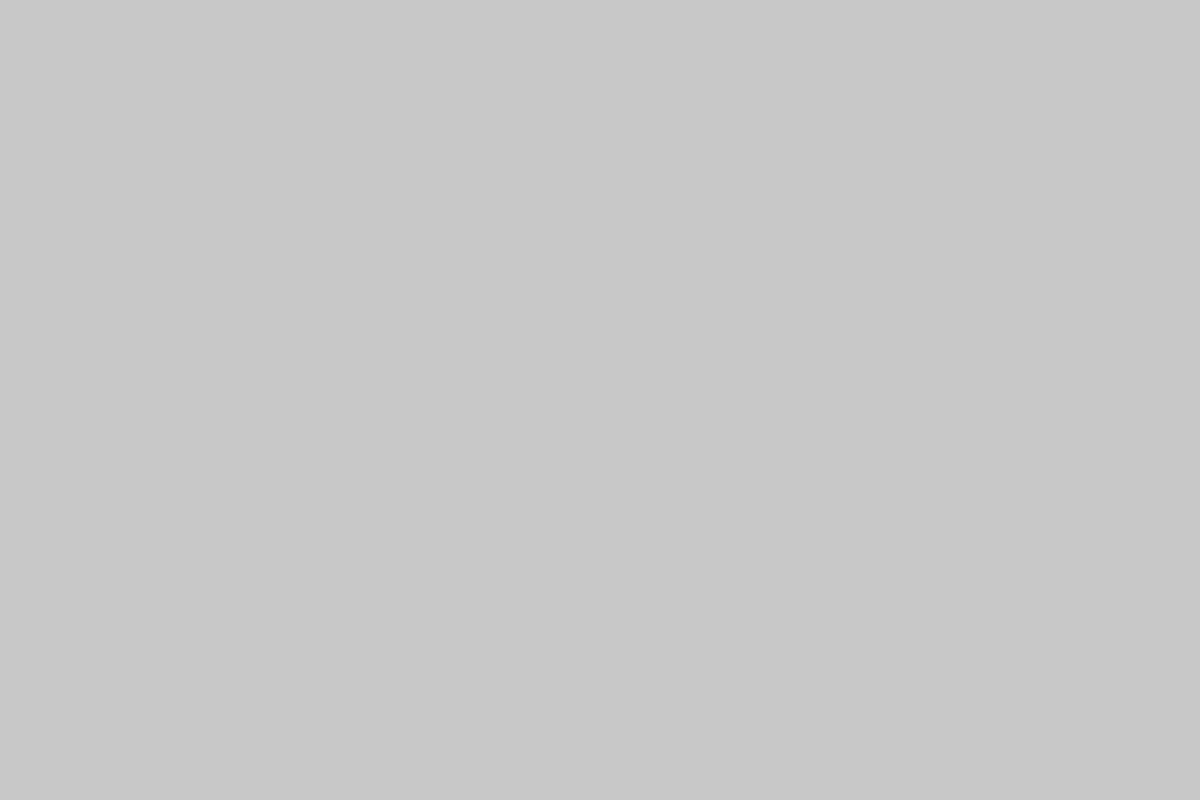
\includegraphics[width=0.9\textwidth]{images/ss-20-dt-viz-code.jpg}}
\caption{Kode visualisasi perbandingan 50 nilai aktual dan prediksi Decision Tree.}
\label{fig:ss20-dtvizcode}
\end{figure}

\begin{figure}[H]
\centering
\customfbox{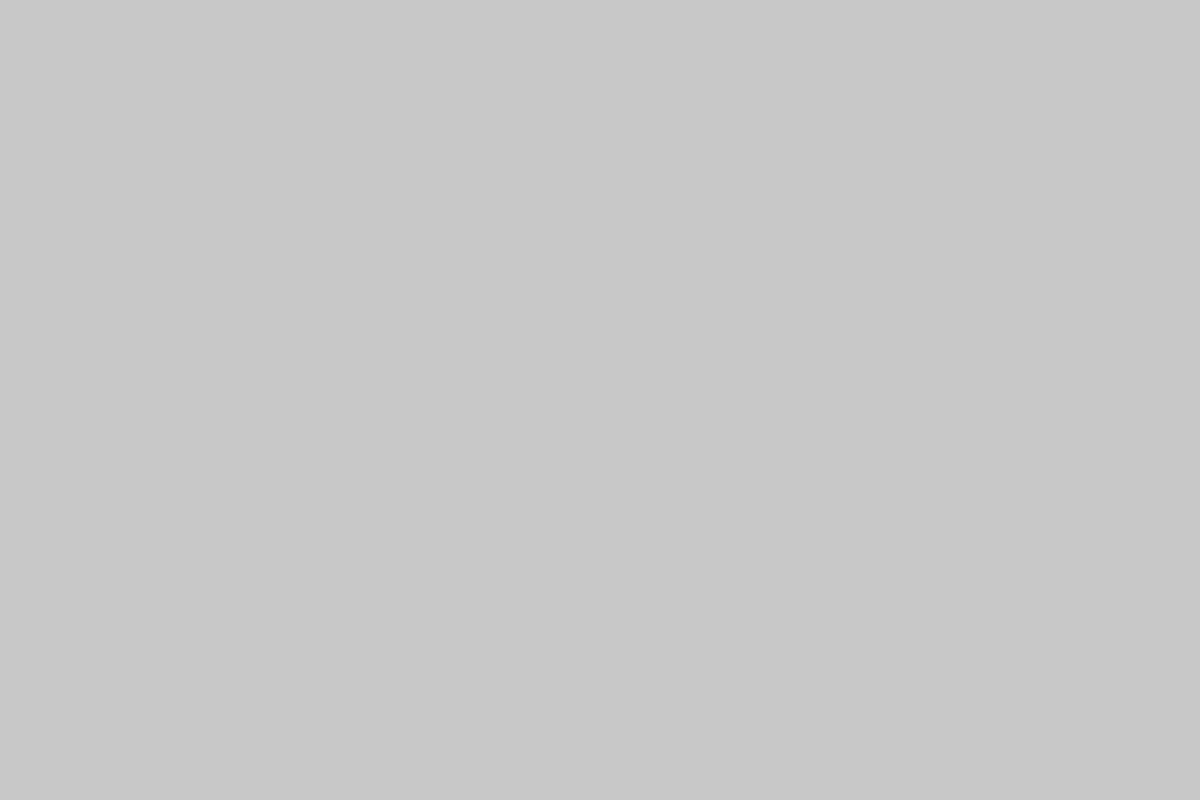
\includegraphics[width=0.9\textwidth]{images/ss-21-dt-viz-result.jpg}}
\caption{Grafik batang perbandingan \texttt{real values} dan \texttt{predicted values} untuk Decision Tree.}
\label{fig:ss21-dtvizres}
\end{figure}

\subsubsection{c. Random Forest Regression}
Untuk Random Forest, langkahnya sama dengan inisialisasi \texttt{RandomForestRegressor()} memakai parameter default, yang secara default membangun sekumpulan pohon keputusan dan merata-ratakan prediksinya.

\begin{lstlisting}[style=pythonstyle,caption={Kode model Random Forest Regression.}]
from sklearn.ensemble import RandomForestRegressor
from sklearn.model_selection import train_test_split

df_X = df.drop(['id','date','price'], axis=1)
df_y = df['price']

X = df_X.astype(float).values
y = df_y.astype(float).values

X_train, X_test, y_train, y_test = train_test_split(X, y, test_size=0.3, random_state=42)

rf = RandomForestRegressor()
rf.fit(X_train, y_train)

print('coef of determination training', rf.score(X_train, y_train))
print('coef of determination testing', rf.score(X_test, y_test))

print('prediction')
y_pred = rf.predict(X_test)
print(y_pred[:10])
print('real value')
print(y_test[0:10])
\end{lstlisting}

\begin{figure}[H]
\centering
\customfbox{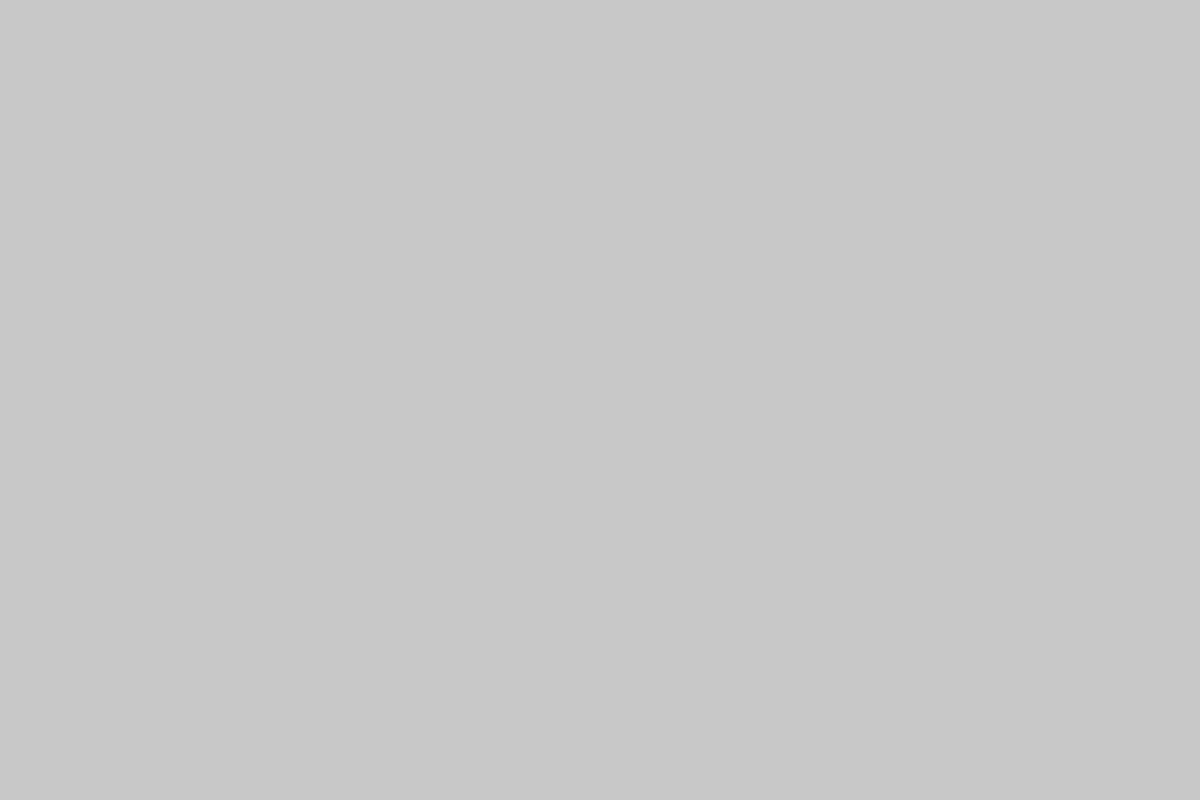
\includegraphics[width=0.9\textwidth]{images/ss-22-rf-code.jpg}}
\caption{Kode pemodelan Random Forest Regression dengan parameter default.}
\label{fig:ss22-rfcode}
\end{figure}

Hasilnya R\textsuperscript{2} training 0,9821 berbanding testing 0,8572. Nilai training yang sangat tinggi wajar untuk ensemble, dan yang penting skor testingnya tetap yang tertinggi di antara ketiga model, artinya generalisasinya terbaik.

\begin{figure}[H]
\centering
\customfbox{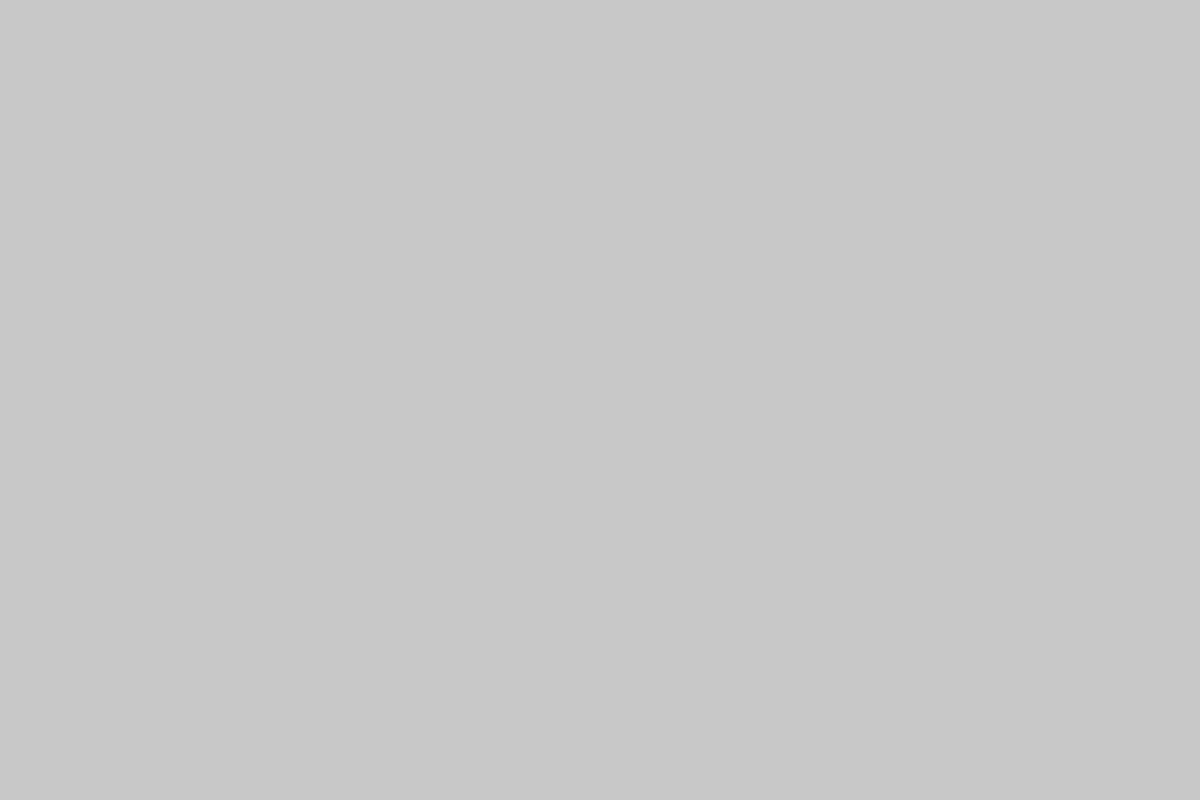
\includegraphics[width=0.9\textwidth]{images/ss-23-rf-output.jpg}}
\caption{Output pelatihan dan prediksi Random Forest Regression.}
\label{fig:ss23-rfout}
\end{figure}

\begin{lstlisting}[style=pythonstyle,caption={Kode evaluasi Random Forest.}]
from sklearn.metrics import mean_squared_error
from sklearn.metrics import r2_score
import numpy as np

mse = mean_squared_error(y_test, y_pred)
rmse = np.sqrt(mse)
r2 = r2_score(y_test, y_pred)

print('rmse:', rmse)
print('r2:', r2)
\end{lstlisting}

\begin{figure}[H]
\centering
\customfbox{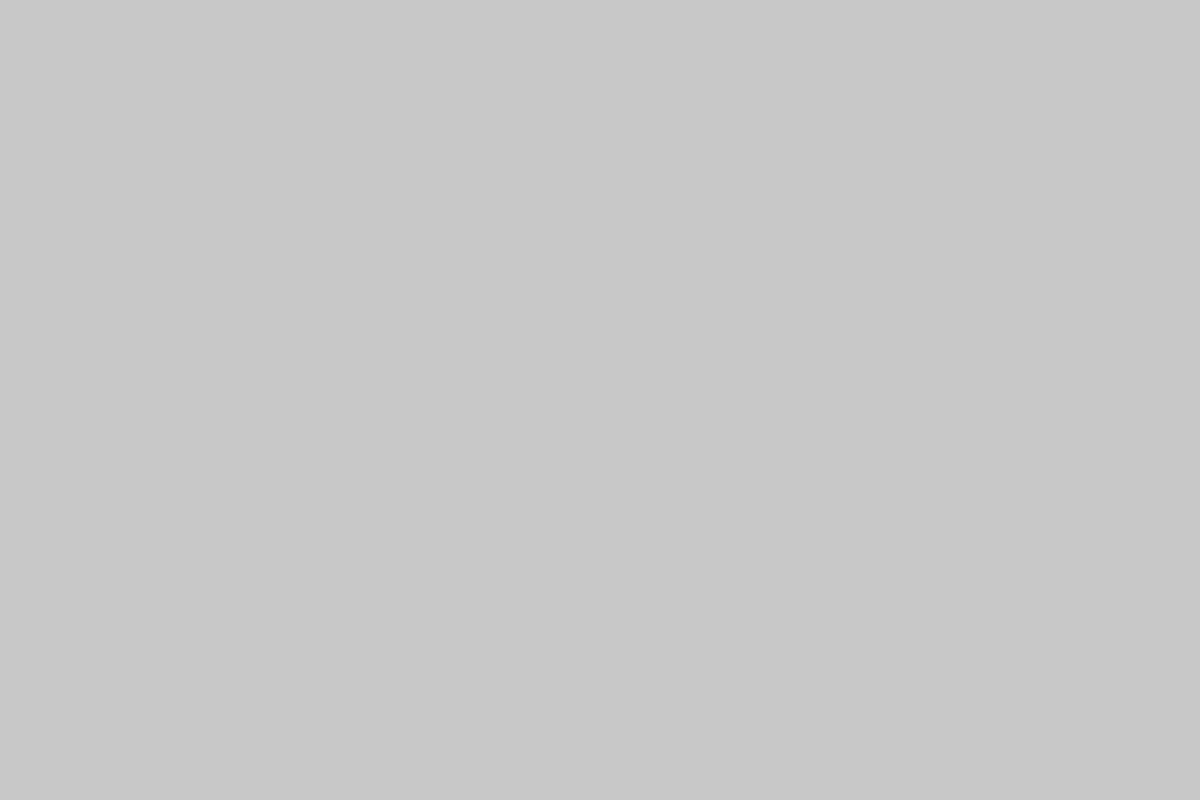
\includegraphics[width=0.7\textwidth]{images/ss-24-rf-eval-code.jpg}}
\caption{Kode evaluasi Random Forest menggunakan RMSE dan R\textsuperscript{2}.}
\label{fig:ss24-rfevalcode}
\end{figure}

Hasilnya RMSE 143.577,64 dan R\textsuperscript{2} 0,8572: RMSE terendah dan R\textsuperscript{2} tertinggi di antara ketiga model, membuktikan keunggulan metode ensemble dalam menangkap pola data yang kompleks.

\begin{figure}[H]
\centering
\customfbox{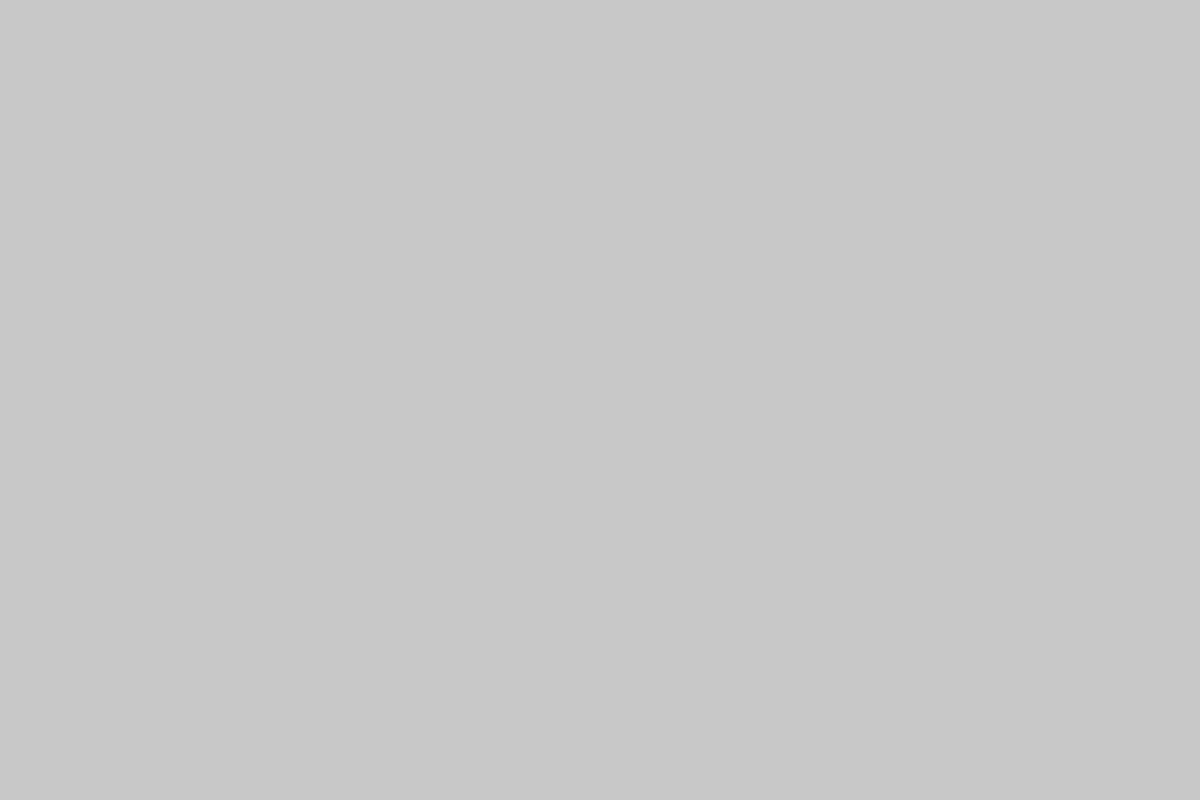
\includegraphics[width=0.7\textwidth]{images/ss-25-rf-eval-result.jpg}}
\caption{Hasil evaluasi Random Forest: RMSE terendah dan R\textsuperscript{2} tertinggi.}
\label{fig:ss25-rfevalres}
\end{figure}

\begin{lstlisting}[style=pythonstyle,caption={Kode visualisasi Random Forest.}]
import seaborn as sns
import matplotlib.pyplot as plt

data1 = pd.Series(y_test[:50].ravel())
data2 = pd.Series(y_pred[:50].ravel())

df_new = pd.concat([data1, data2], keys=['real values', 'predicted values'], axis=1)
df_new.plot(kind='bar', figsize=(15,3))

plt.title("RF regression")
plt.xlabel('Sample i')
plt.ylabel('House Price')
plt.show()
\end{lstlisting}

\begin{figure}[H]
\centering
\customfbox{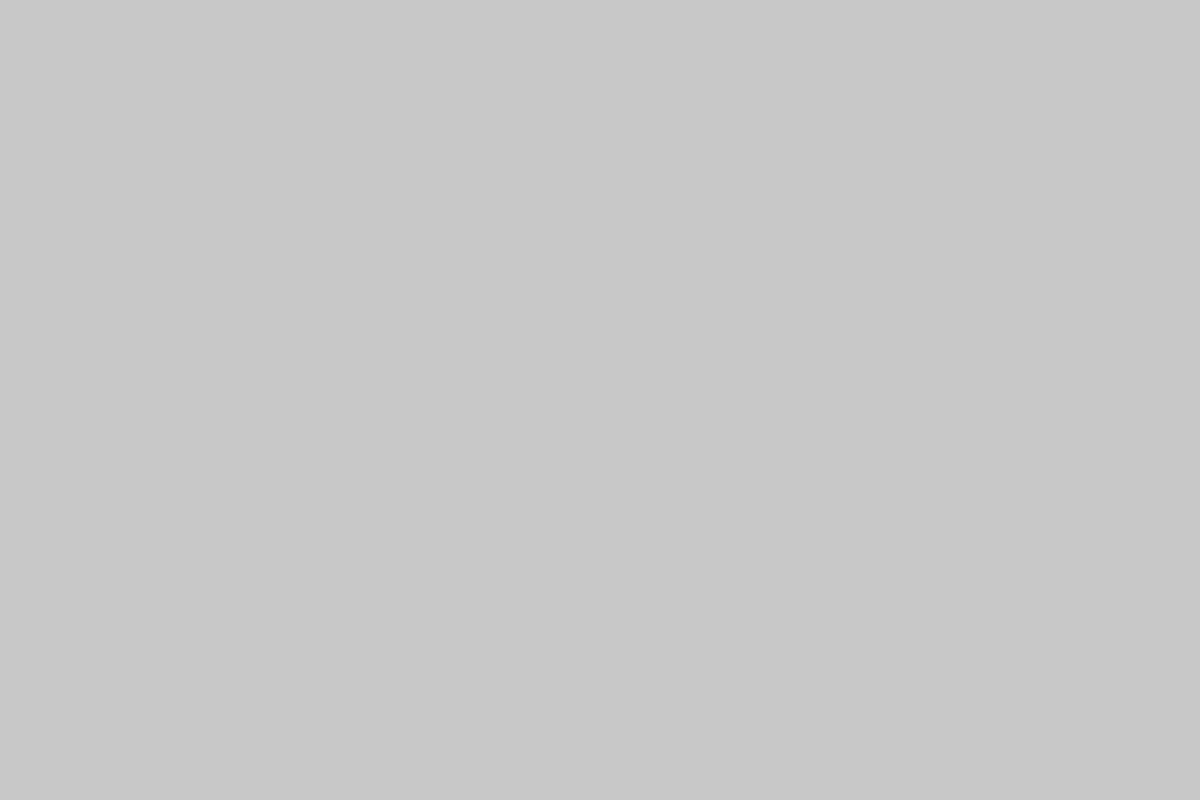
\includegraphics[width=0.9\textwidth]{images/ss-26-rf-viz-code.jpg}}
\caption{Kode visualisasi perbandingan 50 nilai aktual dan prediksi Random Forest.}
\label{fig:ss26-rfvizcode}
\end{figure}

\begin{figure}[H]
\centering
\customfbox{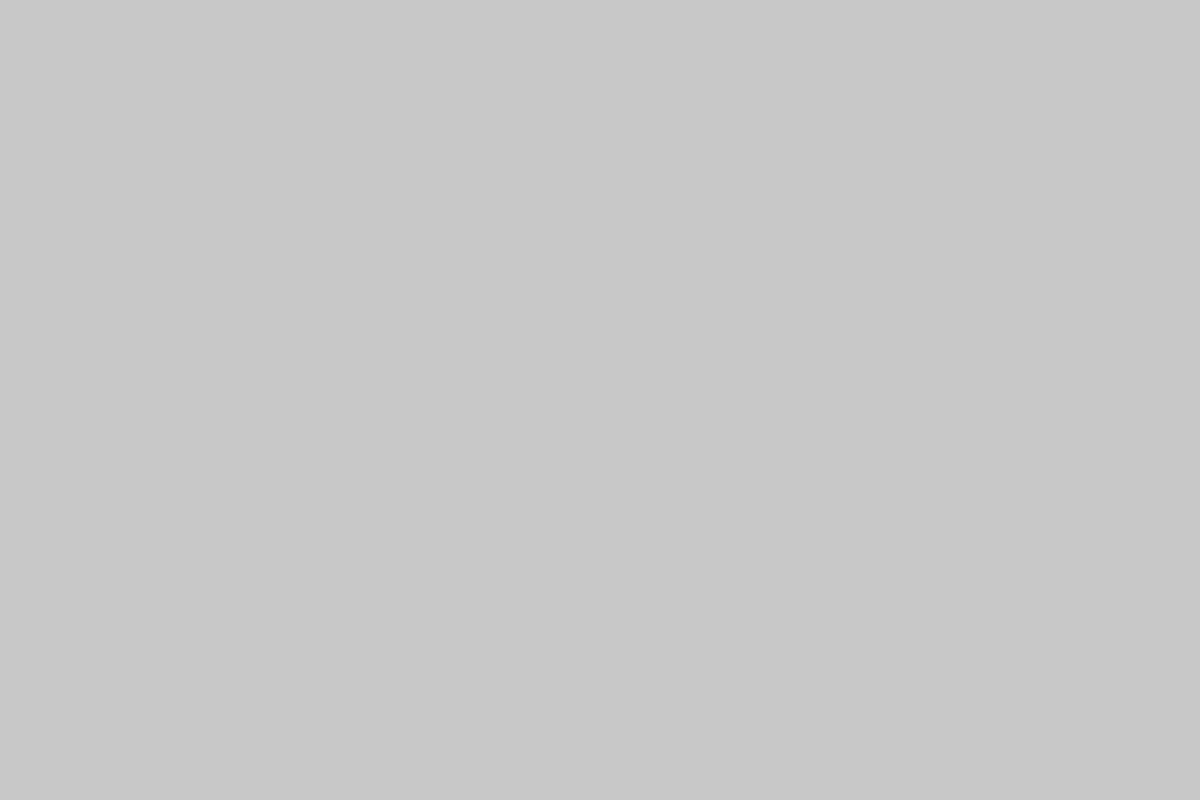
\includegraphics[width=0.9\textwidth]{images/ss-27-rf-viz-result.jpg}}
\caption{Grafik batang perbandingan \texttt{real values} dan \texttt{predicted values} untuk Random Forest: batang prediksi hampir berimpit dengan nilai sebenarnya.}
\label{fig:ss27-rfvizres}
\end{figure}

\subsection{Perbandingan Performa Model KC House}
Ringkasan hasil eksperimen ketiga model pada dataset KC House (verifikasi lokal Python 3.11, scikit-learn 1.9.0, split 70:30) saya susun pada Tabel~\ref{tab:performa-kc}.

\begin{table}[H]
\centering
\small
\begin{tabular}{lccc}
\toprule
\textbf{Model} & \textbf{RMSE} & \textbf{R2} & \textbf{R} \\
\midrule
Linear Regression & 208296.73 & 0.6995 & 0.8365 \\
Decision Tree (max\_depth=10) & 184751.00 & 0.7636 & 0.8727 \\
Random Forest & 143577.64 & 0.8572 & 0.9243 \\
\bottomrule
\end{tabular}
\caption{Perbandingan performa tiga model regresi pada dataset KC House.}
\label{tab:performa-kc}
\end{table}

Pola yang terlihat konsisten: Random Forest terbaik di semua metrik, Decision Tree di tengah, dan Linear Regression paling rendah. Hal ini wajar karena hubungan harga rumah terhadap fiturnya banyak yang non-linear (interaksi luas, grade, lokasi), sehingga model pohon yang fleksibel mengungguli garis linier. Selisih R\textsuperscript{2} training dan testing juga memberi pelajaran: Linear Regression hampir tidak overfitting (0,6995 vs 0,6995), sedangkan Decision Tree (0,9185 vs 0,7586) dan Random Forest (0,9821 vs 0,8572) menunjukkan gap yang wajar untuk model berkapasitas besar.

\subsection{Tugas dan Analisis: Car Price Prediction}
Sesuai Modul 4.5, saya mengerjakan tugas tambahan menggunakan dataset \textit{Car Price Prediction} (\url{https://www.kaggle.com/datasets/hellbuoy/car-price-prediction/data}).

\subsubsection{Tujuan Penggunaan Dataset}
Dataset Car Price Prediction digunakan untuk memprediksi harga mobil berdasarkan spesifikasi teknisnya, agar perusahaan konsultan otomotif dapat menetapkan harga jual yang kompetitif tanpa harus melakukan survei manual untuk setiap unit. Dataset klasik ini (205 baris, 26 kolom) juga sering dipakai sebagai studi kasus regresi linier berganda karena menggabungkan fitur numerik (dimensi, mesin, konsumsi BBM) dan kategorikal (jenis bahan bakar, bodi, penggerak) \cite{kaggle-car,car-mirror}.

\subsubsection{Atribut Input dan Output}
Berdasarkan eksplorasi awal dataset, atribut dapat didefinisikan sebagai berikut:
\begin{itemize}
    \item \textbf{Atribut input (fitur):} seluruh kolom kecuali \texttt{price} --- dimensi (\texttt{wheelbase}, \texttt{carlength}, \texttt{carwidth}, \texttt{carheight}, \texttt{curbweight}), mesin (\texttt{enginesize}, \texttt{boreratio}, \texttt{stroke}, \texttt{compressionratio}, \texttt{horsepower}, \texttt{peakrpm}), konsumsi BBM (\texttt{citympg}, \texttt{highwaympg}), simbol risiko (\texttt{symboling}), serta kolom kategorikal (\texttt{fueltype}, \texttt{aspiration}, \texttt{doornumber}, \texttt{carbody}, \texttt{drivewheel}, \texttt{enginelocation}, \texttt{enginetype}, \texttt{cylindernumber}, \texttt{fuelsystem}) yang saya encoding. Kolom \texttt{car\_ID} dan \texttt{CarName} saya buang sebagai identifier/nama unit yang tidak general.
    \item \textbf{Atribut output (target):} \texttt{price} (harga mobil, kontinu; rata-rata 13.276,71, rentang 5.118--45.400).
\end{itemize}

\begin{table}[H]
\centering
\small
\begin{tabular}{|l|p{9cm}|}
\hline
\textbf{Atribut} & \textbf{Penjelasan} \\
\hline
\texttt{car\_ID} & Identifier unik unit mobil (dibuang saat pemodelan). \\
\texttt{symboling} & Tingkat risiko asuransi mobil. \\
\texttt{CarName} & Nama/merek unit mobil (dibuang, terlalu spesifik). \\
\texttt{fueltype} & Jenis bahan bakar (gas/diesel). \\
\texttt{aspiration} & Tipe aspirasi mesin (std/turbo). \\
\texttt{doornumber} & Jumlah pintu (two/four). \\
\texttt{carbody} & Bentuk bodi (sedan/hatchback/wagon/dsb). \\
\texttt{drivewheel} & Penggerak roda (fwd/rwd/4wd). \\
\texttt{enginelocation} & Posisi mesin (front/rear). \\
\texttt{wheelbase}, \texttt{carlength}, \texttt{carwidth}, \texttt{carheight}, \texttt{curbweight} & Dimensi dan bobot mobil. \\
\texttt{enginetype}, \texttt{cylindernumber}, \texttt{enginesize}, \texttt{fuelsystem} & Spesifikasi mesin dan sistem bahan bakar. \\
\texttt{boreratio}, \texttt{stroke}, \texttt{compressionratio}, \texttt{horsepower}, \texttt{peakrpm} & Parameter performa mesin. \\
\texttt{citympg}, \texttt{highwaympg} & Konsumsi BBM dalam kota dan jalan tol. \\
\texttt{price} & Target: harga mobil (kontinu). \\
\hline
\end{tabular}
\caption{Deskripsi atribut dataset Car Price Prediction.}
\label{tab:car-attributes}
\end{table}

\subsubsection{Eksplorasi Awal dan Preprocessing Dataset Car}
Saya memuat dataset dari mirror GitHub dan melakukan EDA singkat: memeriksa head, info, deskripsi statistik, dan korelasi. Tidak ada missing value di seluruh kolom. Korelasi tertinggi dengan \texttt{price} adalah \texttt{enginesize} (0,87), \texttt{curbweight} (0,84), dan \texttt{horsepower} (0,81) --- spesifikasi mesin dan bobot paling menentukan harga mobil.

\begin{lstlisting}[style=pythonstyle,caption={Memuat dan memeriksa dataset Car.}]
car_url = 'https://raw.githubusercontent.com/SampattKumar/Linear-Regression-Car-Dataset/master/CarPrice_Assignment.csv' # mirror GitHub dari Kaggle
car_df = pd.read_csv(car_url)
print(car_df.shape)  # (205, 26)
print(car_df.head())
print(car_df.info())
print(car_df.describe())
print(car_df.isnull().sum())  # 0 missing di semua kolom
print(car_df.corr(numeric_only=True)['price'].drop('price').sort_values(ascending=False).head(6))
\end{lstlisting}

\begin{figure}[H]
\centering
\customfbox{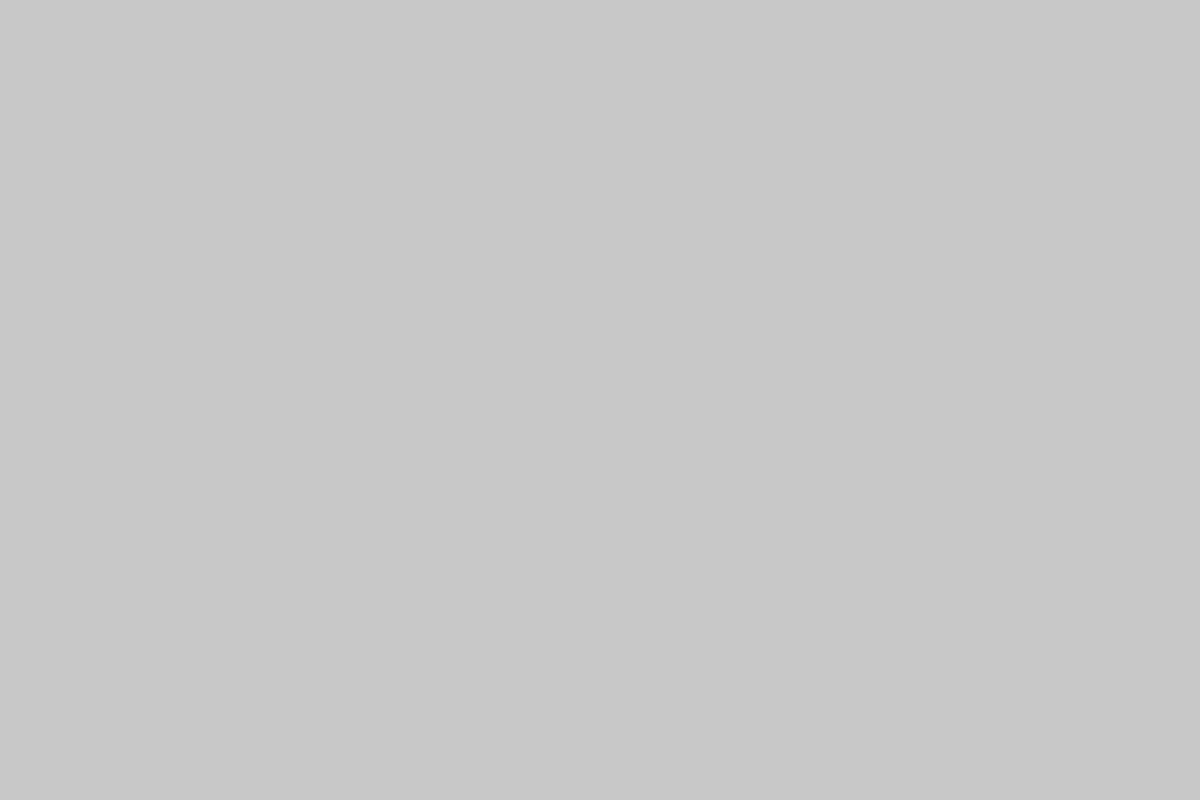
\includegraphics[width=0.9\textwidth]{images/ss-tugas-01-car-head.jpg}}
\caption{Lima baris pertama dataset Car Price beserta info kolom.}
\label{fig:tugas01-car-head}
\end{figure}

\begin{figure}[H]
\centering
\customfbox{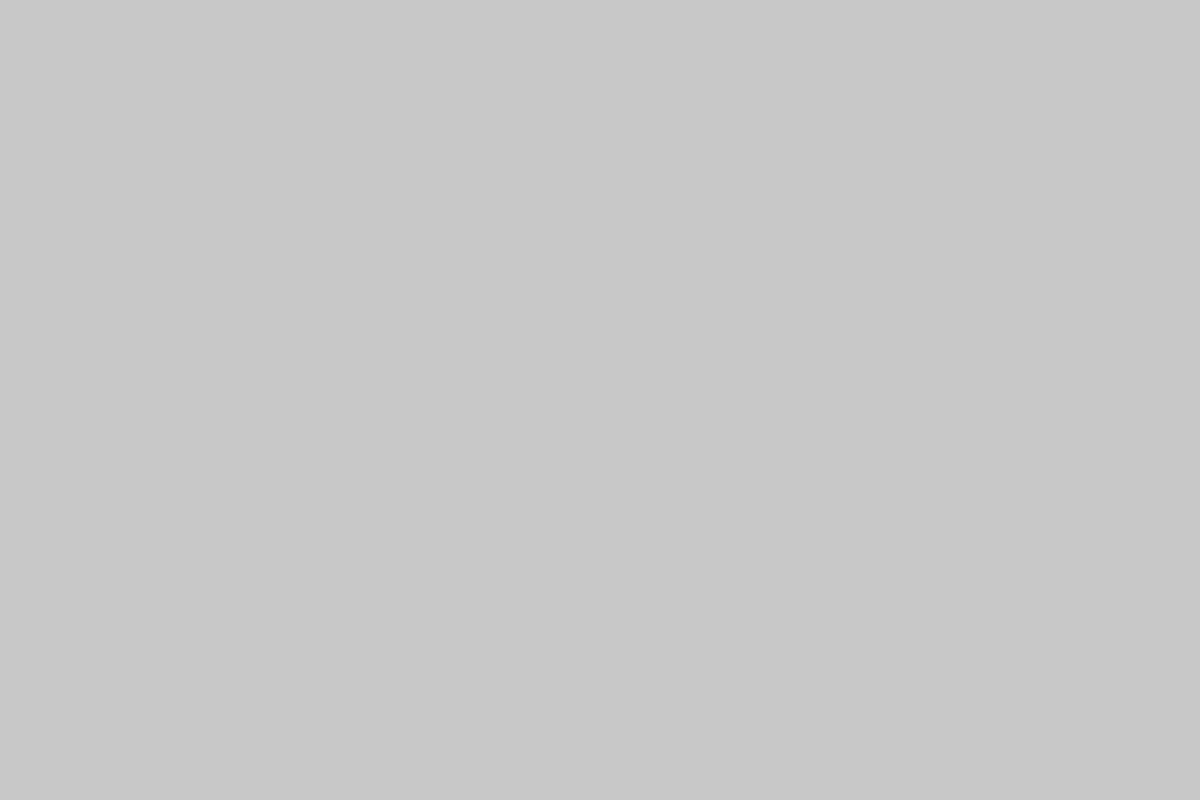
\includegraphics[width=0.9\textwidth]{images/ss-tugas-02-car-eda.jpg}}
\caption{Hasil EDA dataset Car: deskripsi statistik dan korelasi tertinggi terhadap \texttt{price} (\texttt{enginesize}, \texttt{curbweight}, \texttt{horsepower}).}
\label{fig:tugas02-car-eda}
\end{figure}

Untuk preprocessing, saya melakukan: (1) membuang \texttt{car\_ID} dan \texttt{CarName}, (2) \textit{one-hot encoding} kolom kategorikal dengan \texttt{pd.get\_dummies(drop\_first=True)} yang menghasilkan 43 fitur numerik, (3) split 70:30, dan (4) StandardScaler yang di-fit hanya pada data train --- konsisten dengan workflow P3 yang memakai \texttt{.astype(int)} setelah \texttt{get\_dummies} agar kolom boolean tidak menghasilkan NaN saat scaling.

\begin{lstlisting}[style=pythonstyle,caption={Preprocessing dataset Car.}]
from sklearn.preprocessing import StandardScaler

car2 = car_df.drop(['car_ID', 'CarName'], axis=1)
X_car = pd.get_dummies(car2.drop(['price'], axis=1), drop_first=True).astype(int)
y_car = car2['price'].astype(float).values  # hasil: (205, 43) fitur numerik
print('X_car shape:', X_car.shape)

X_train_c, X_test_c, y_train_c, y_test_c = train_test_split(X_car.values, y_car, test_size=0.3, random_state=42)
scaler_c = StandardScaler().fit(X_train_c)
X_train_cs = scaler_c.transform(X_train_c)
X_test_cs = scaler_c.transform(X_test_c)
print('mean train ~0:', X_train_cs.mean().round(6))
\end{lstlisting}

\begin{figure}[H]
\centering
\customfbox{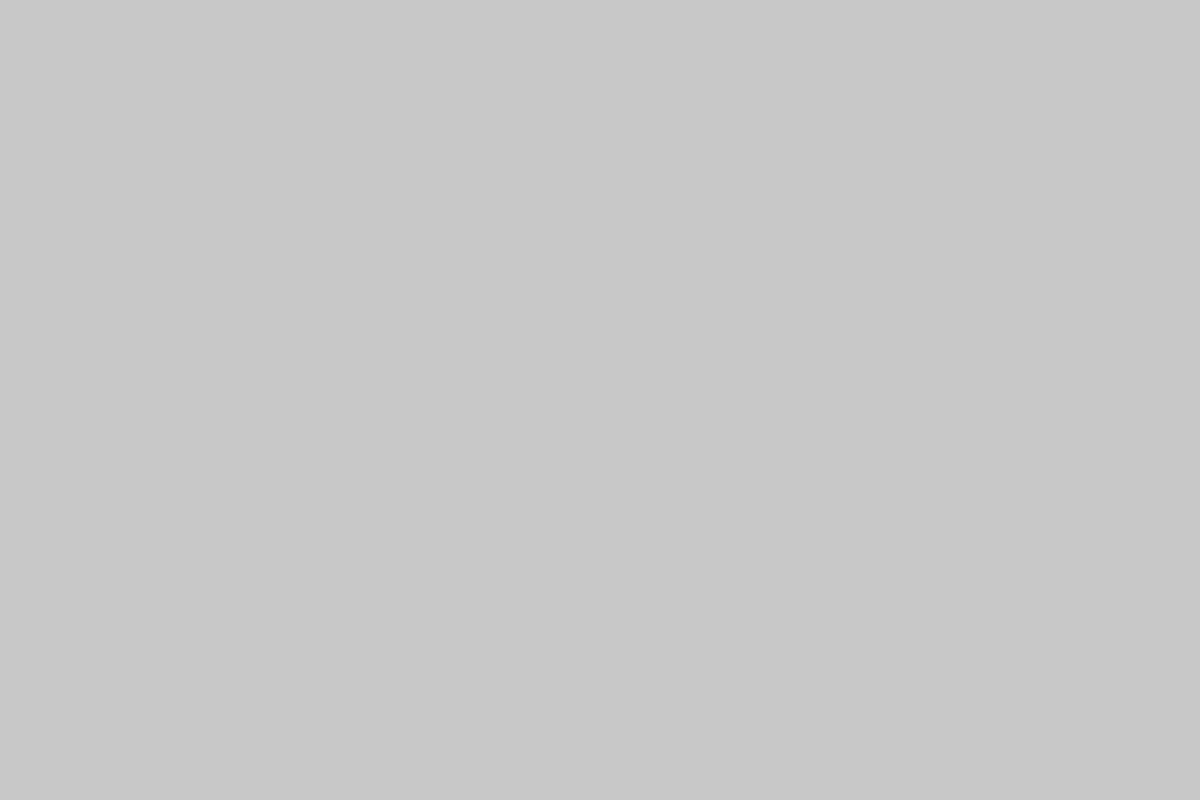
\includegraphics[width=0.9\textwidth]{images/ss-tugas-03-car-preprocessing.jpg}}
\caption{Hasil preprocessing dataset Car: bentuk fitur (205, 43) dan hasil scaling dengan mean mendekati nol.}
\label{fig:tugas03-car-preprocess}
\end{figure}

\subsubsection{Pemodelan Regresi pada Dataset Car}

\textbf{Linear Regression:}
\begin{lstlisting}[style=pythonstyle,caption={Linear Regression pada dataset Car.}]
model = LinearRegression()
model.fit(X_train_cs, y_train_c)
y_pred_c = model.predict(X_test_cs)
rmse_c = np.sqrt(mean_squared_error(y_test_c, y_pred_c))
r2_c = r2_score(y_test_c, y_pred_c)
r_c = np.corrcoef(y_test_c, y_pred_c)[0, 1]
print('train R2:', model.score(X_train_cs, y_train_c))
print('test R2:', model.score(X_test_cs, y_test_c))
print('rmse:', rmse_c)
print('r2:', r2_c)
print('r:', r_c)
\end{lstlisting}

\begin{figure}[H]
\centering
\customfbox{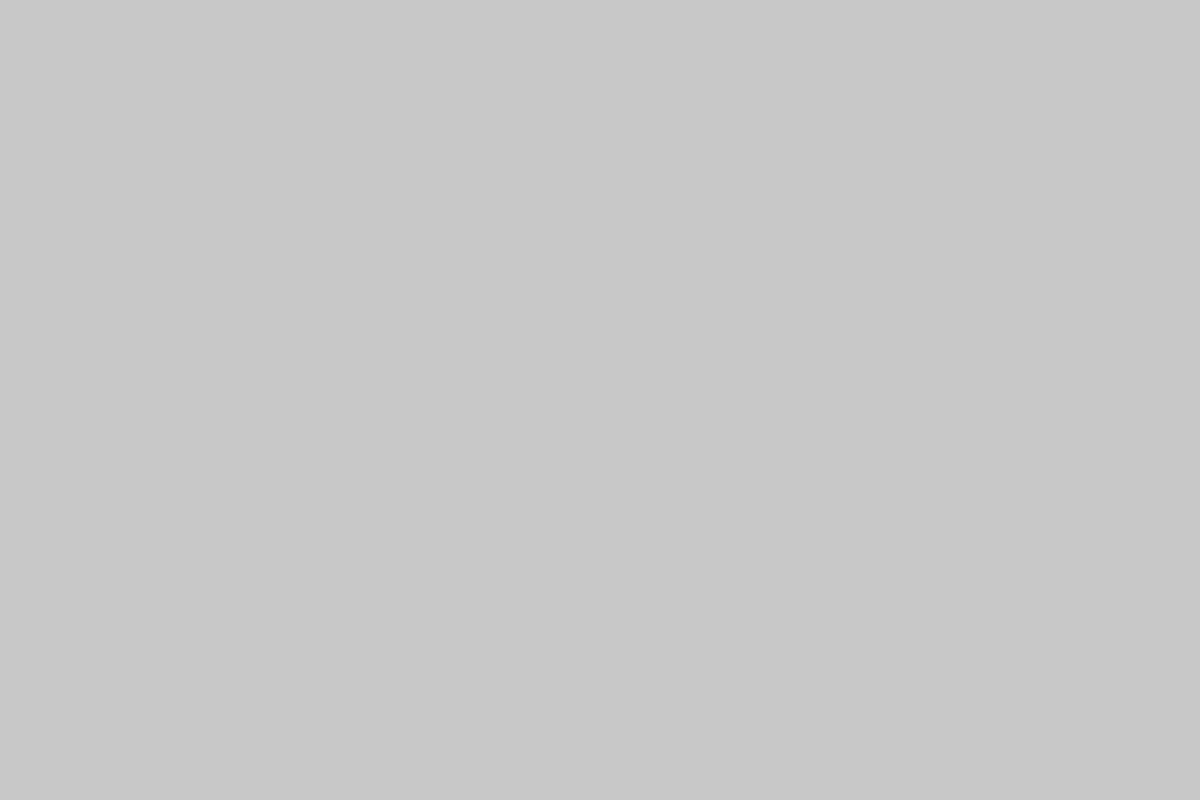
\includegraphics[width=0.9\textwidth]{images/ss-tugas-04-car-linear.jpg}}
\caption{Performa Linear Regression pada dataset Car (RMSE 2854,60, R2 0,8824).}
\label{fig:tugas04-linear}
\end{figure}

\textbf{Decision Tree (max\_depth=10):}
\begin{lstlisting}[style=pythonstyle,caption={Decision Tree pada dataset Car.}]
model = DecisionTreeRegressor(max_depth=10, random_state=42)
model.fit(X_train_cs, y_train_c)
y_pred_c = model.predict(X_test_cs)
rmse_c = np.sqrt(mean_squared_error(y_test_c, y_pred_c))
r2_c = r2_score(y_test_c, y_pred_c)
r_c = np.corrcoef(y_test_c, y_pred_c)[0, 1]
print('train R2:', model.score(X_train_cs, y_train_c))
print('test R2:', model.score(X_test_cs, y_test_c))
print('rmse:', rmse_c)
print('r2:', r2_c)
print('r:', r_c)
\end{lstlisting}

\begin{figure}[H]
\centering
\customfbox{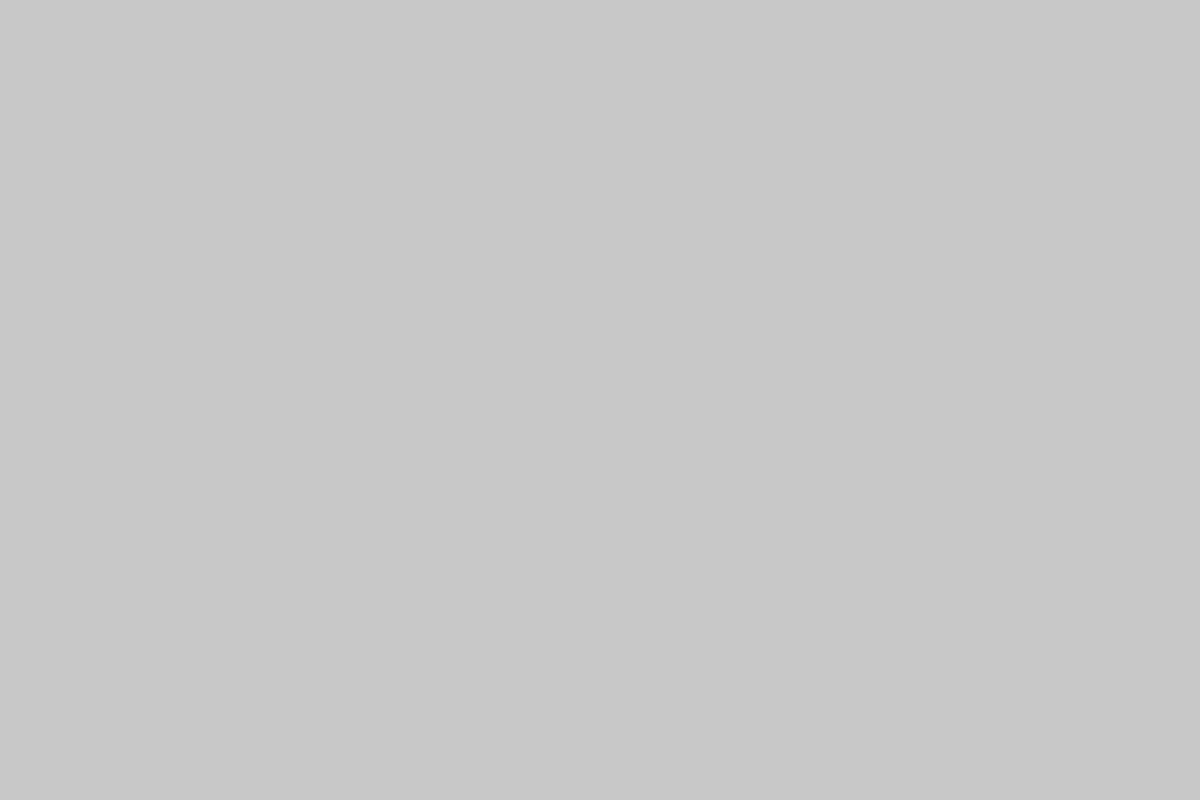
\includegraphics[width=0.9\textwidth]{images/ss-tugas-05-car-dt.jpg}}
\caption{Performa Decision Tree pada dataset Car (RMSE 2822,67, R2 0,8850).}
\label{fig:tugas05-dt}
\end{figure}

\textbf{Random Forest:}
\begin{lstlisting}[style=pythonstyle,caption={Random Forest pada dataset Car.}]
model = RandomForestRegressor(random_state=42)
model.fit(X_train_cs, y_train_c)
y_pred_c = model.predict(X_test_cs)
rmse_c = np.sqrt(mean_squared_error(y_test_c, y_pred_c))
r2_c = r2_score(y_test_c, y_pred_c)
r_c = np.corrcoef(y_test_c, y_pred_c)[0, 1]
print('train R2:', model.score(X_train_cs, y_train_c))
print('test R2:', model.score(X_test_cs, y_test_c))
print('rmse:', rmse_c)
print('r2:', r2_c)
print('r:', r_c)
\end{lstlisting}

\begin{figure}[H]
\centering
\customfbox{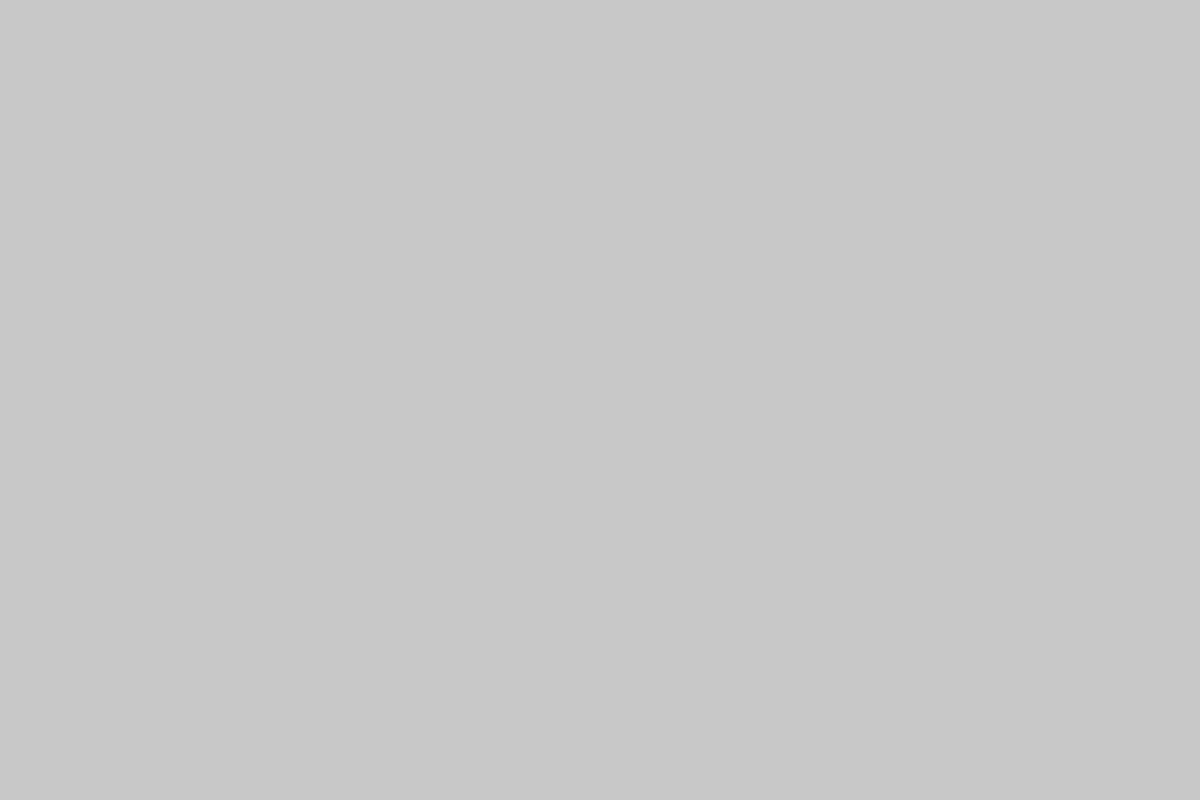
\includegraphics[width=0.9\textwidth]{images/ss-tugas-06-car-rf.jpg}}
\caption{Performa Random Forest pada dataset Car (RMSE 1984,06, R2 0,9432).}
\label{fig:tugas06-rf}
\end{figure}

\subsubsection{Tabel Performa Model}

\begin{lstlisting}[style=pythonstyle,caption={Tabel performa model Car.}]
from sklearn.metrics import mean_squared_error, r2_score

results = []
configs = [
    ('Linear Regression', LinearRegression()),
    ('Decision Tree (max_depth=10)', DecisionTreeRegressor(max_depth=10, random_state=42)),
    ('Random Forest', RandomForestRegressor(random_state=42)),
]
for name, m in configs:
    m.fit(X_train_cs, y_train_c)
    yp = m.predict(X_test_cs)
    results.append({'model': name, 'RMSE': np.sqrt(mean_squared_error(y_test_c, yp)), 'R2': r2_score(y_test_c, yp), 'R': np.corrcoef(y_test_c, yp)[0, 1]})
perf = pd.DataFrame(results)
display(perf)
\end{lstlisting}

\begin{table}[H]
\centering
\small
\begin{tabular}{lccc}
\toprule
\textbf{Model} & \textbf{RMSE} & \textbf{R2} & \textbf{R} \\
\midrule
Linear Regression & 2854.60 & 0.8824 & 0.9400 \\
Decision Tree (max\_depth=10) & 2822.67 & 0.8850 & 0.9510 \\
Random Forest & 1984.06 & 0.9432 & 0.9720 \\
\bottomrule
\end{tabular}
\caption{Perbandingan performa tiga model regresi pada dataset Car Price Prediction (hasil verifikasi lokal Python 3.11, scikit-learn 1.9.0, split 70:30, StandardScaler).}
\label{tab:performa-car}
\end{table}

\begin{figure}[H]
\centering
\customfbox{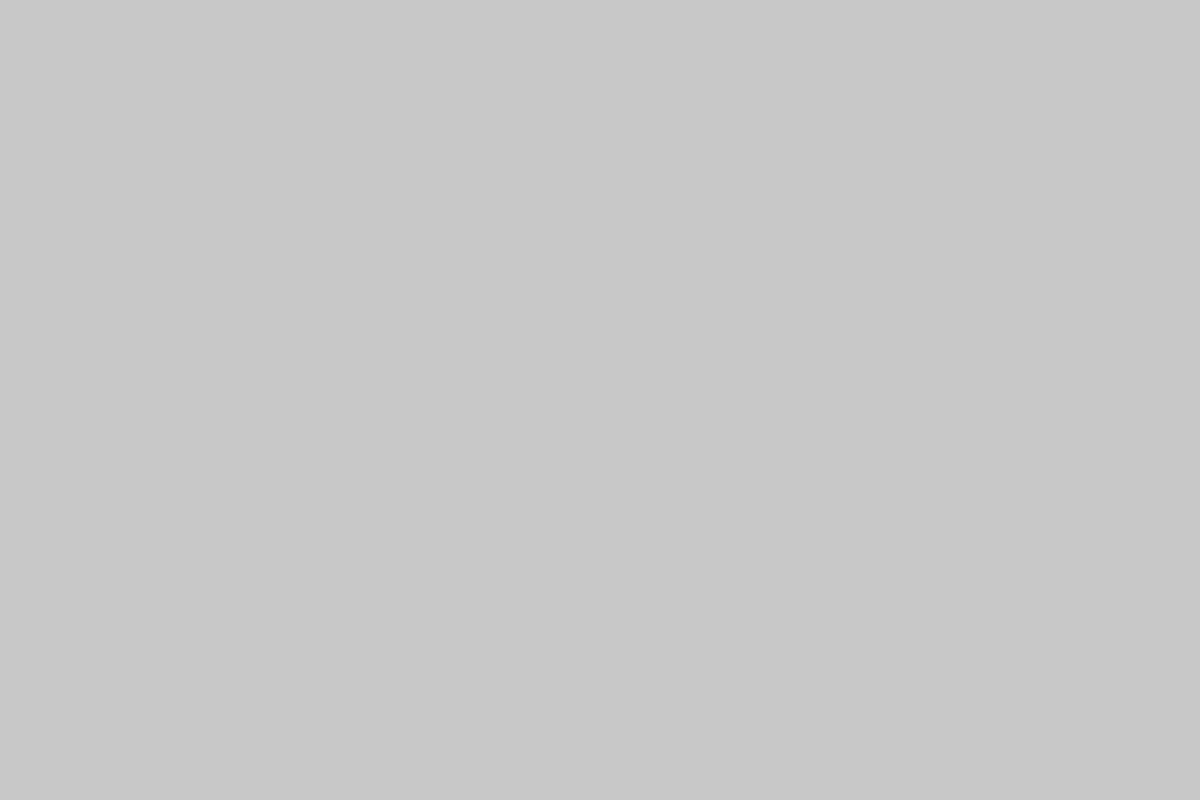
\includegraphics[width=0.9\textwidth]{images/ss-tugas-07-car-tabel-performa.jpg}}
\caption{Tabel performa model yang dihasilkan dari kode Python (output DataFrame).}
\label{fig:tugas07-tabel}
\end{figure}

\subsubsection{Analisis Model Terbaik}
Berdasarkan eksperimen pada dataset Car (Tabel~\ref{tab:performa-car}), model \textbf{Random Forest} menunjukkan performa terbaik secara keseluruhan dengan RMSE terendah 1.984,06, R2 tertinggi 0,9432, dan korelasi R tertinggi 0,9720. Keunggulan ini konsisten dengan karakteristik ensemble yang merata-ratakan banyak pohon sehingga meredam variansi pohon tunggal dan menangkap interaksi non-linear antar spesifikasi mobil. Decision Tree berada di posisi kedua (RMSE 2.822,67, R2 0,8850) dan Linear Regression ketiga (RMSE 2.854,60, R2 0,8824); selisih keduanya tipis karena hubungan harga mobil terhadap spesifikasi seperti \texttt{enginesize} dan \texttt{curbweight} memang cenderung linear, sehingga model sederhana sudah kompetitif, namun ensemble tetap menang dengan margin yang jelas.

Pola yang sama terlihat pada percobaan KC House (Tabel~\ref{tab:performa-kc}): Random Forest terbaik (RMSE 143.577,64, R2 0,8572), diikuti Decision Tree (RMSE 184.751,00, R2 0,7636), dan Linear Regression terakhir (RMSE 208.296,73, R2 0,6995). Dengan demikian, pada kedua dataset, Random Forest adalah pilihan terbaik dengan alasan yang sama: kemampuan ensemble menangkap pola kompleks tanpa mengorbankan generalisasi.

\clearpage

\chapter{Kesimpulan}
Berdasarkan praktikum yang telah saya lakukan pada Pertemuan 4, saya memahami beberapa hal berikut:
\begin{enumerate}
    \item Regresi adalah teknik supervised learning untuk memprediksi target numerik yang kontinu. Saya telah memahami konsep dasarnya: model mempelajari fungsi matematis dari pasangan input--output berlabel untuk memprediksi nilai baru, berbeda dengan klasifikasi yang keluarannya label diskrit dan clustering yang tidak memakai label.
    \item Saya telah mempelajari prinsip kerja tiga algoritma regresi: Linear Regression (membangun garis/hyperplane terbaik dengan Least Squares yang meminimalkan SSE, cepat dan interpretable tetapi terbatas pada pola linear dan sensitif terhadap outlier), Decision Tree Regression (membagi data secara rekursif berdasarkan split yang meminimalkan MSE, efektif untuk pola non-linear tetapi rawan overfitting sehingga perlu \texttt{max\_depth} atau pruning), dan Random Forest Regression (ensemble bootstrap yang merata-ratakan banyak pohon sehingga stabil, akurat, dan memberi feature importance dengan biaya komputasi lebih besar).
    \item Saya berhasil menerapkan ketiga algoritma tersebut pada dataset KC House (21.613 baris, 21 kolom) dengan workflow yang benar: EDA (deskripsi statistik, histogram, korelasi, cek missing value, cek kategorikal), pemisahan fitur/target dengan membuang \texttt{id} dan \texttt{date}, konversi float, dan split 70:30 dengan \texttt{random\_state=42}.
    \item Evaluasi model dengan RMSE, R\textsuperscript{2}, dan korelasi R menunjukkan hasil yang konsisten pada kedua dataset: pada KC House, Random Forest terbaik (RMSE 143.577,64, R2 0,8572, R 0,9243), diikuti Decision Tree (RMSE 184.751,00, R2 0,7636), dan Linear Regression (RMSE 208.296,73, R2 0,6995); pada tugas Car Price Prediction, Random Forest juga terbaik (RMSE 1.984,06, R2 0,9432, R 0,9720). Saya juga memahami mengapa accuracy/precision/recall tidak dipakai untuk regresi: metrik tersebut membutuhkan konsep benar/salah dari target diskrit, sedangkan prediksi regresi bersifat kontinu sehingga kualitasnya harus diukur dari besarnya error (RMSE) dan proporsi variansi yang dijelaskan (R\textsuperscript{2}).
\end{enumerate}
Dengan demikian, praktikum ini memberikan dasar yang penting bagi saya untuk memilih, melatih, dan mengevaluasi model regresi secara objektif, tidak hanya melihat satu metrik tetapi mempertimbangkan RMSE, R\textsuperscript{2}, dan korelasi secara bersamaan.

\clearpage
\addcontentsline{toc}{chapter}{Daftar Pustaka}
\renewcommand{\bibname}{Daftar Pustaka}
\begin{thebibliography}{99}
    \bibitem{han2022} J. Han, J. Pei, and H. Tong, \textit{Data Mining: Concepts and Techniques}, 4th ed. Morgan Kaufmann/Elsevier, 2022.

    \bibitem{python-docs} Python Software Foundation, ``Python 3 Documentation.'' [Online]. Tersedia: \url{https://www.python.org/doc/}.

    \bibitem{pandas-docs} The pandas Development Team, ``pandas.DataFrame.'' [Online]. Tersedia: \url{https://pandas.pydata.org/docs/reference/api/pandas.DataFrame.html}.

    \bibitem{numpy-docs} NumPy Developers, ``NumPy Documentation.'' [Online]. Tersedia: \url{https://numpy.org/}.

    \bibitem{sklearn-linear} Scikit-learn Developers, ``Linear Models.'' [Online]. Tersedia: \url{https://scikit-learn.org/stable/modules/linear_model.html}.

    \bibitem{sklearn-tree} Scikit-learn Developers, ``Decision Trees.'' [Online]. Tersedia: \url{https://scikit-learn.org/stable/modules/tree.html}.

    \bibitem{sklearn-ensemble} Scikit-learn Developers, ``Ensemble methods.'' [Online]. Tersedia: \url{https://scikit-learn.org/stable/modules/ensemble.html}.

    \bibitem{sklearn-metrics} Scikit-learn Developers, ``Metrics and scoring: quantifying the quality of predictions.'' [Online]. Tersedia: \url{https://scikit-learn.org/stable/modules/model_evaluation.html}.

    \bibitem{sklearn-preprocessing} Scikit-learn Developers, ``Preprocessing data.'' [Online]. Tersedia: \url{https://scikit-learn.org/stable/modules/preprocessing.html}.

    \bibitem{ibm-eda} IBM, ``Apa Itu Analisis Data Eksplorasi?'' [Online]. Tersedia: \url{https://www.ibm.com/id-id/think/topics/exploratory-data-analysis}.

    \bibitem{aws-linear} Amazon Web Services, ``Apa itu Regresi Linier?'' [Online]. Tersedia: \url{https://aws.amazon.com/id/what-is/linear-regression/}.

    \bibitem{kaggle-kc} S. Chandel, ``KC House Data.'' Kaggle. [Online]. Tersedia: \url{https://www.kaggle.com/datasets/shivachandel/kc-house-data}.

    \bibitem{kaggle-car} Hellbuoy, ``Car Price Prediction.'' Kaggle. [Online]. Tersedia: \url{https://www.kaggle.com/datasets/hellbuoy/car-price-prediction/data}.

    \bibitem{car-mirror} S. Kumar, ``Linear Regression Car Dataset (CarPrice\_Assignment.csv).'' GitHub. [Online]. Tersedia: \url{https://github.com/SampattKumar/Linear-Regression-Car-Dataset/blob/master/CarPrice_Assignment.csv}.

    \bibitem{dicoding-regresi} Dicoding Indonesia, ``Rangkuman Supervised Learning - Regresi.'' [Online]. Tersedia: \url{https://www.dicoding.com/academies/184/tutorials/38833}.

    \bibitem{dicoding-workflow} Dicoding Indonesia, ``Machine Learning Workflow: Di Balik Model AI yang Sukses,'' 23 Oktober 2024. [Online]. Tersedia: \url{https://www.dicoding.com/blog/machine-learning-workflow-langkah-langkah-praktis-untuk-membangun-model-ai/}.

    \bibitem{trivusi-aimldl} Trivusi, ``Apa Bedanya Artificial Intelligence, Machine Learning, dan Deep Learning?'' 13 Maret 2022. [Online]. Tersedia: \url{https://www.trivusi.web.id/2022/03/perbedaan-ai-ml-dl.html}.

    \bibitem{itbox-algoritma} ITBOX, ``Algoritma Machine Learning: Pengertian, Penerapan, dan Contohnya,'' 23 Februari 2024. [Online]. Tersedia: \url{https://itbox.id/blog/algoritma-machine-learning-pengertian-penerapan-dan-contohnya/}.

    \bibitem{digitalskola-preprocessing} Digital Skola, ``Data Preprocessing: Definisi, Tahapan, dan Implementasinya.'' [Online]. Tersedia: \url{https://digitalskola.com/blog/data-science/data-preprocessing}.

\end{thebibliography}

\end{document}
